\documentclass[envcountsect,dvips]{beamer}

\setbeamertemplate{background canvas}[vertical shading][bottom=yellow!20,top=blue!10]
%\usetheme{Darmstadt}
\usetheme{Warsaw}
%\usefonttheme[onlysmall]{structurebold}

\usepackage{natbib}
\usepackage{bibentry}
\bibliographystyle{plain}
\usepackage{chngcntr}

\usepackage[utf8]{inputenc}
\usepackage{default}
\usepackage{amsmath}
\usepackage{amsfonts}
\usepackage{amssymb}

\usepackage{graphicx}
\usepackage{caption}
\usepackage{subcaption}

\usepackage{color,xcolor,ucs}% para textcolor



\newenvironment<>{varblock}[2][.9\textwidth]{%
  \setlength{\textwidth}{#1}
  \begin{actionenv}#3%
    \def\insertblocktitle{#2}%
    \par%
    \usebeamertemplate{block begin}}
  {\par%
    \usebeamertemplate{block end}%
  \end{actionenv}}

%%%%%%%%%%%%%%%%%%%%%%%%%%%%%%%%%%%%%%%%%%%%%%%%%%%%%%%%%%%%%%%%%%%%%%%%%%
\begin{document}

\title[Pipeline:   ] % (optional, only for long titles)
{Pipeline:}
\subtitle{Conflitos}
\author[Fernando] % (optional, for multiple authors)
{Fernando Pujaico Rivera\inst{1}}
\institute[Universidade Federal de Lavras] % (optional)
{
  \inst{1}%
  Universidade Federal de Lavras
}
\date[2016] % (optional)
{Aula-1 2016}
\subject{Computer Science}
\frame{\titlepage}

%%%%%%%%%%%%%%%%%%%%%%%%%%%%%%%%%%%%%%%%%%%%%%%%%%%%%%%%%%%%%%%%%%%%%%%%%%%%%%%%
%%%%%%%%%%%%%%%%%%%%%%%%%%%%%%%%%%%%%%%%%%%%%%%%%%%%%%%%%%%%%%%%%%%%%%%%%%%%%%%%
%%%%%%%%%%%%%%%%%%%%%%%%%%%%%%%%%%%%%%%%%%%%%%%%%%%%%%%%%%%%%%%%%%%%%%%%%%%%%%%%
\section{Exemplo de pipeline}

% https://www.youtube.com/watch?v=NmDdrI9ALxg
%https://www.youtube.com/watch?v=tcAbPJC_Qhs



%%%%%%%%%%%%%%%%%%%%%%%%%%%%%%%%%%%%%%%%%%%%%%%%%%%%%%%%%%%%%%%%%%%%%%%%%%%%%%%%%
\begin{frame}{Exemplo de pipeline}
\begin{center}
\includegraphics[width=0.9\textwidth]{images/exemplopipe.eps}
\end{center}
\end{frame}

%%%%%%%%%%%%%%%%%%%%%%%%%%%%%%%%%%%%%%%%%%%%%%%%%%%%%%%%%%%%%%%%%%%%%%%%%%%%%%%%%
\begin{frame}{Exemplo de pipeline}
\begin{block}{Divisões}
\begin{description}
 \item[Dois estágios] Fetch e Execute.
 \item[Três estágios] Fetch, {\color{red}Decode} e Execute.
 \item[Cinco estágios] Fetch, Decode, Execute, {\color{red}MemAccess} e {\color{red}Write back}.
\end{description}
Interrupção: Salva o estado atual e processa a Interrupção.
\end{block}
\begin{center}
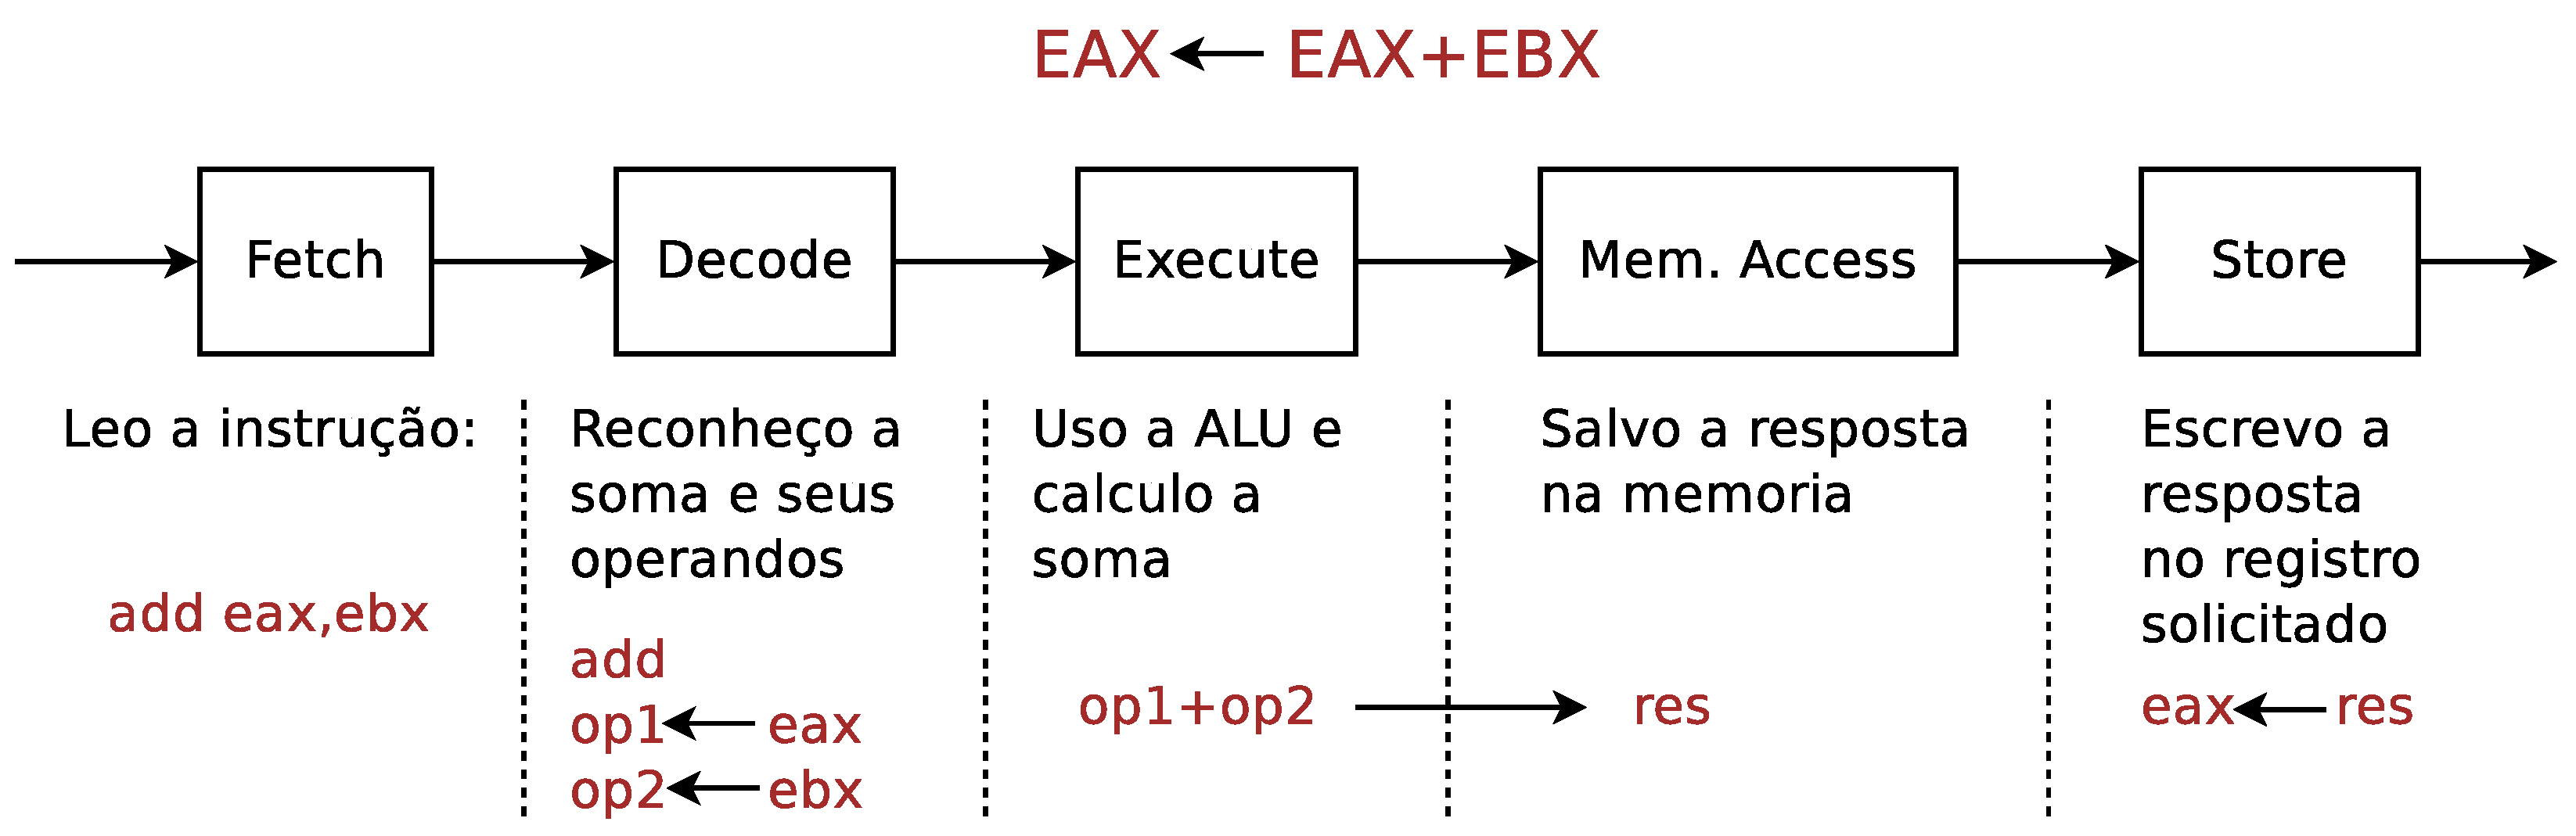
\includegraphics[width=1.0\textwidth]{images/5passos.eps}
\end{center}
\end{frame}

%%%%%%%%%%%%%%%%%%%%%%%%%%%%%%%%%%%%%%%%%%%%%%%%%%%%%%%%%%%%%%%%%%%%%%%%%%%%%%%%%
\begin{frame}{Exemplo de pipeline}
\begin{minipage}[c]{0.5\textwidth}
\begin{center}
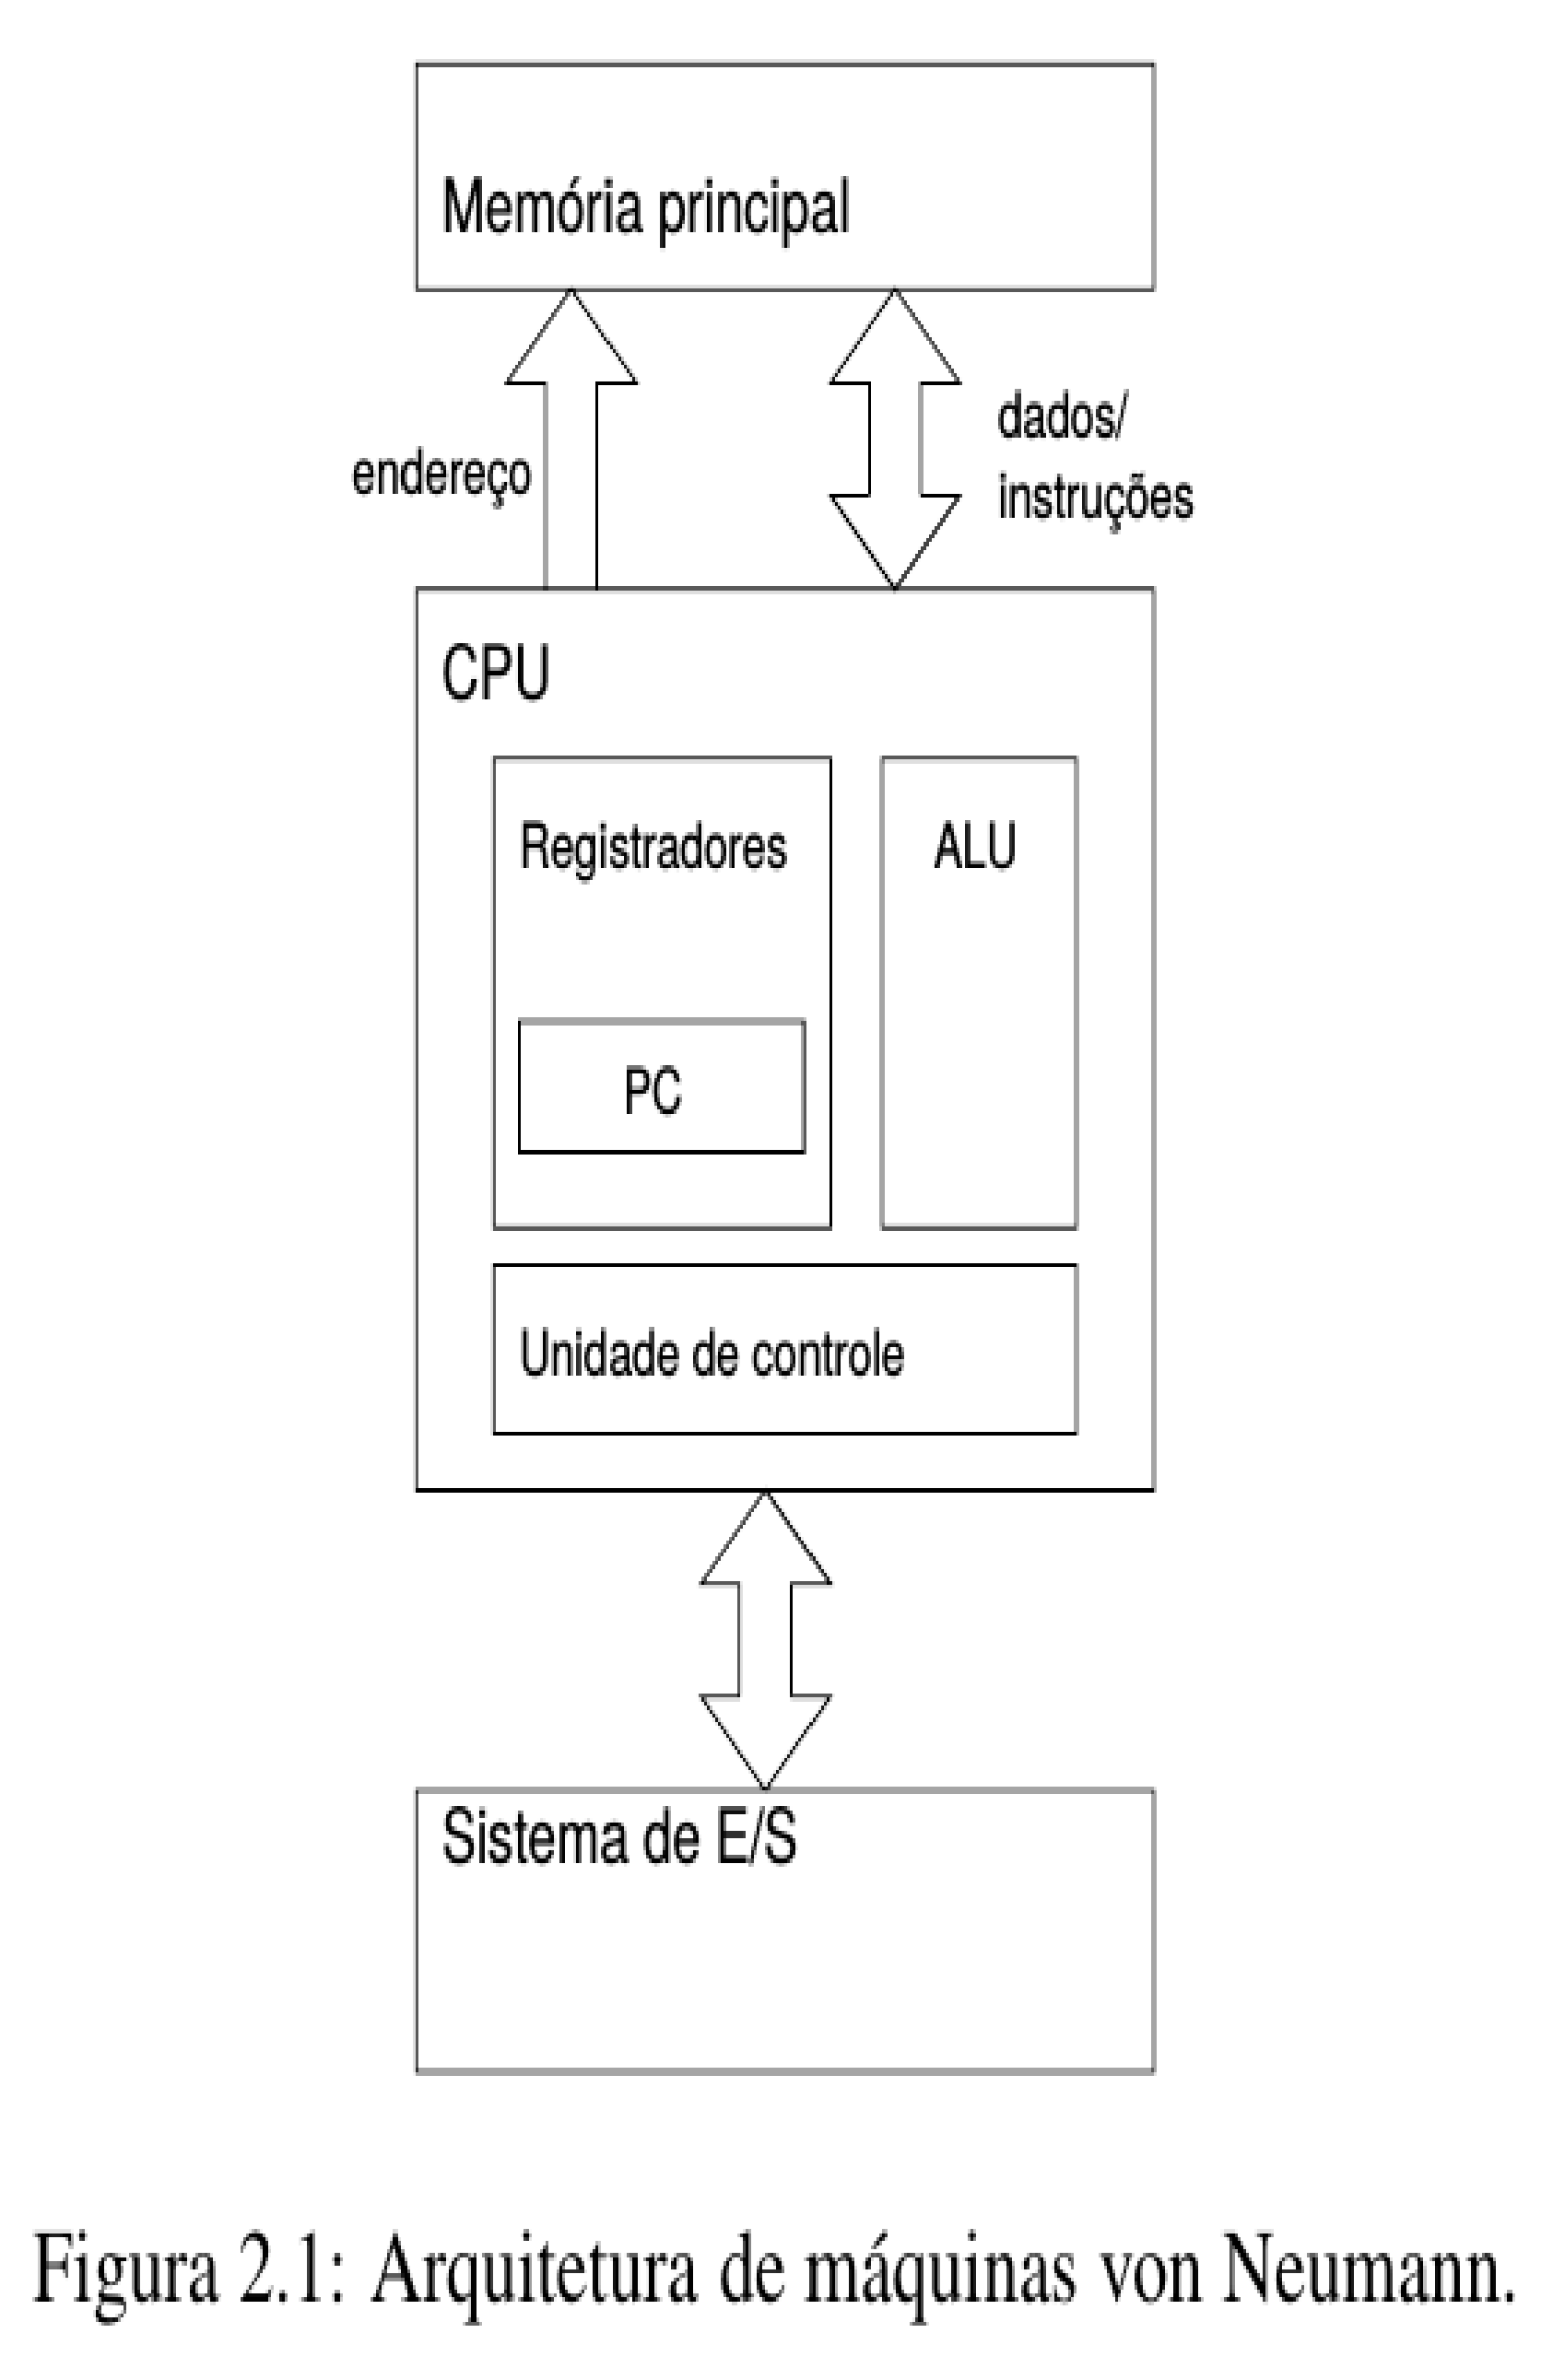
\includegraphics[width=0.8\textwidth]{images/vonnewman1.eps}
\end{center} 
\end{minipage}%
\begin{minipage}[c]{0.5\textwidth}
\begin{center}
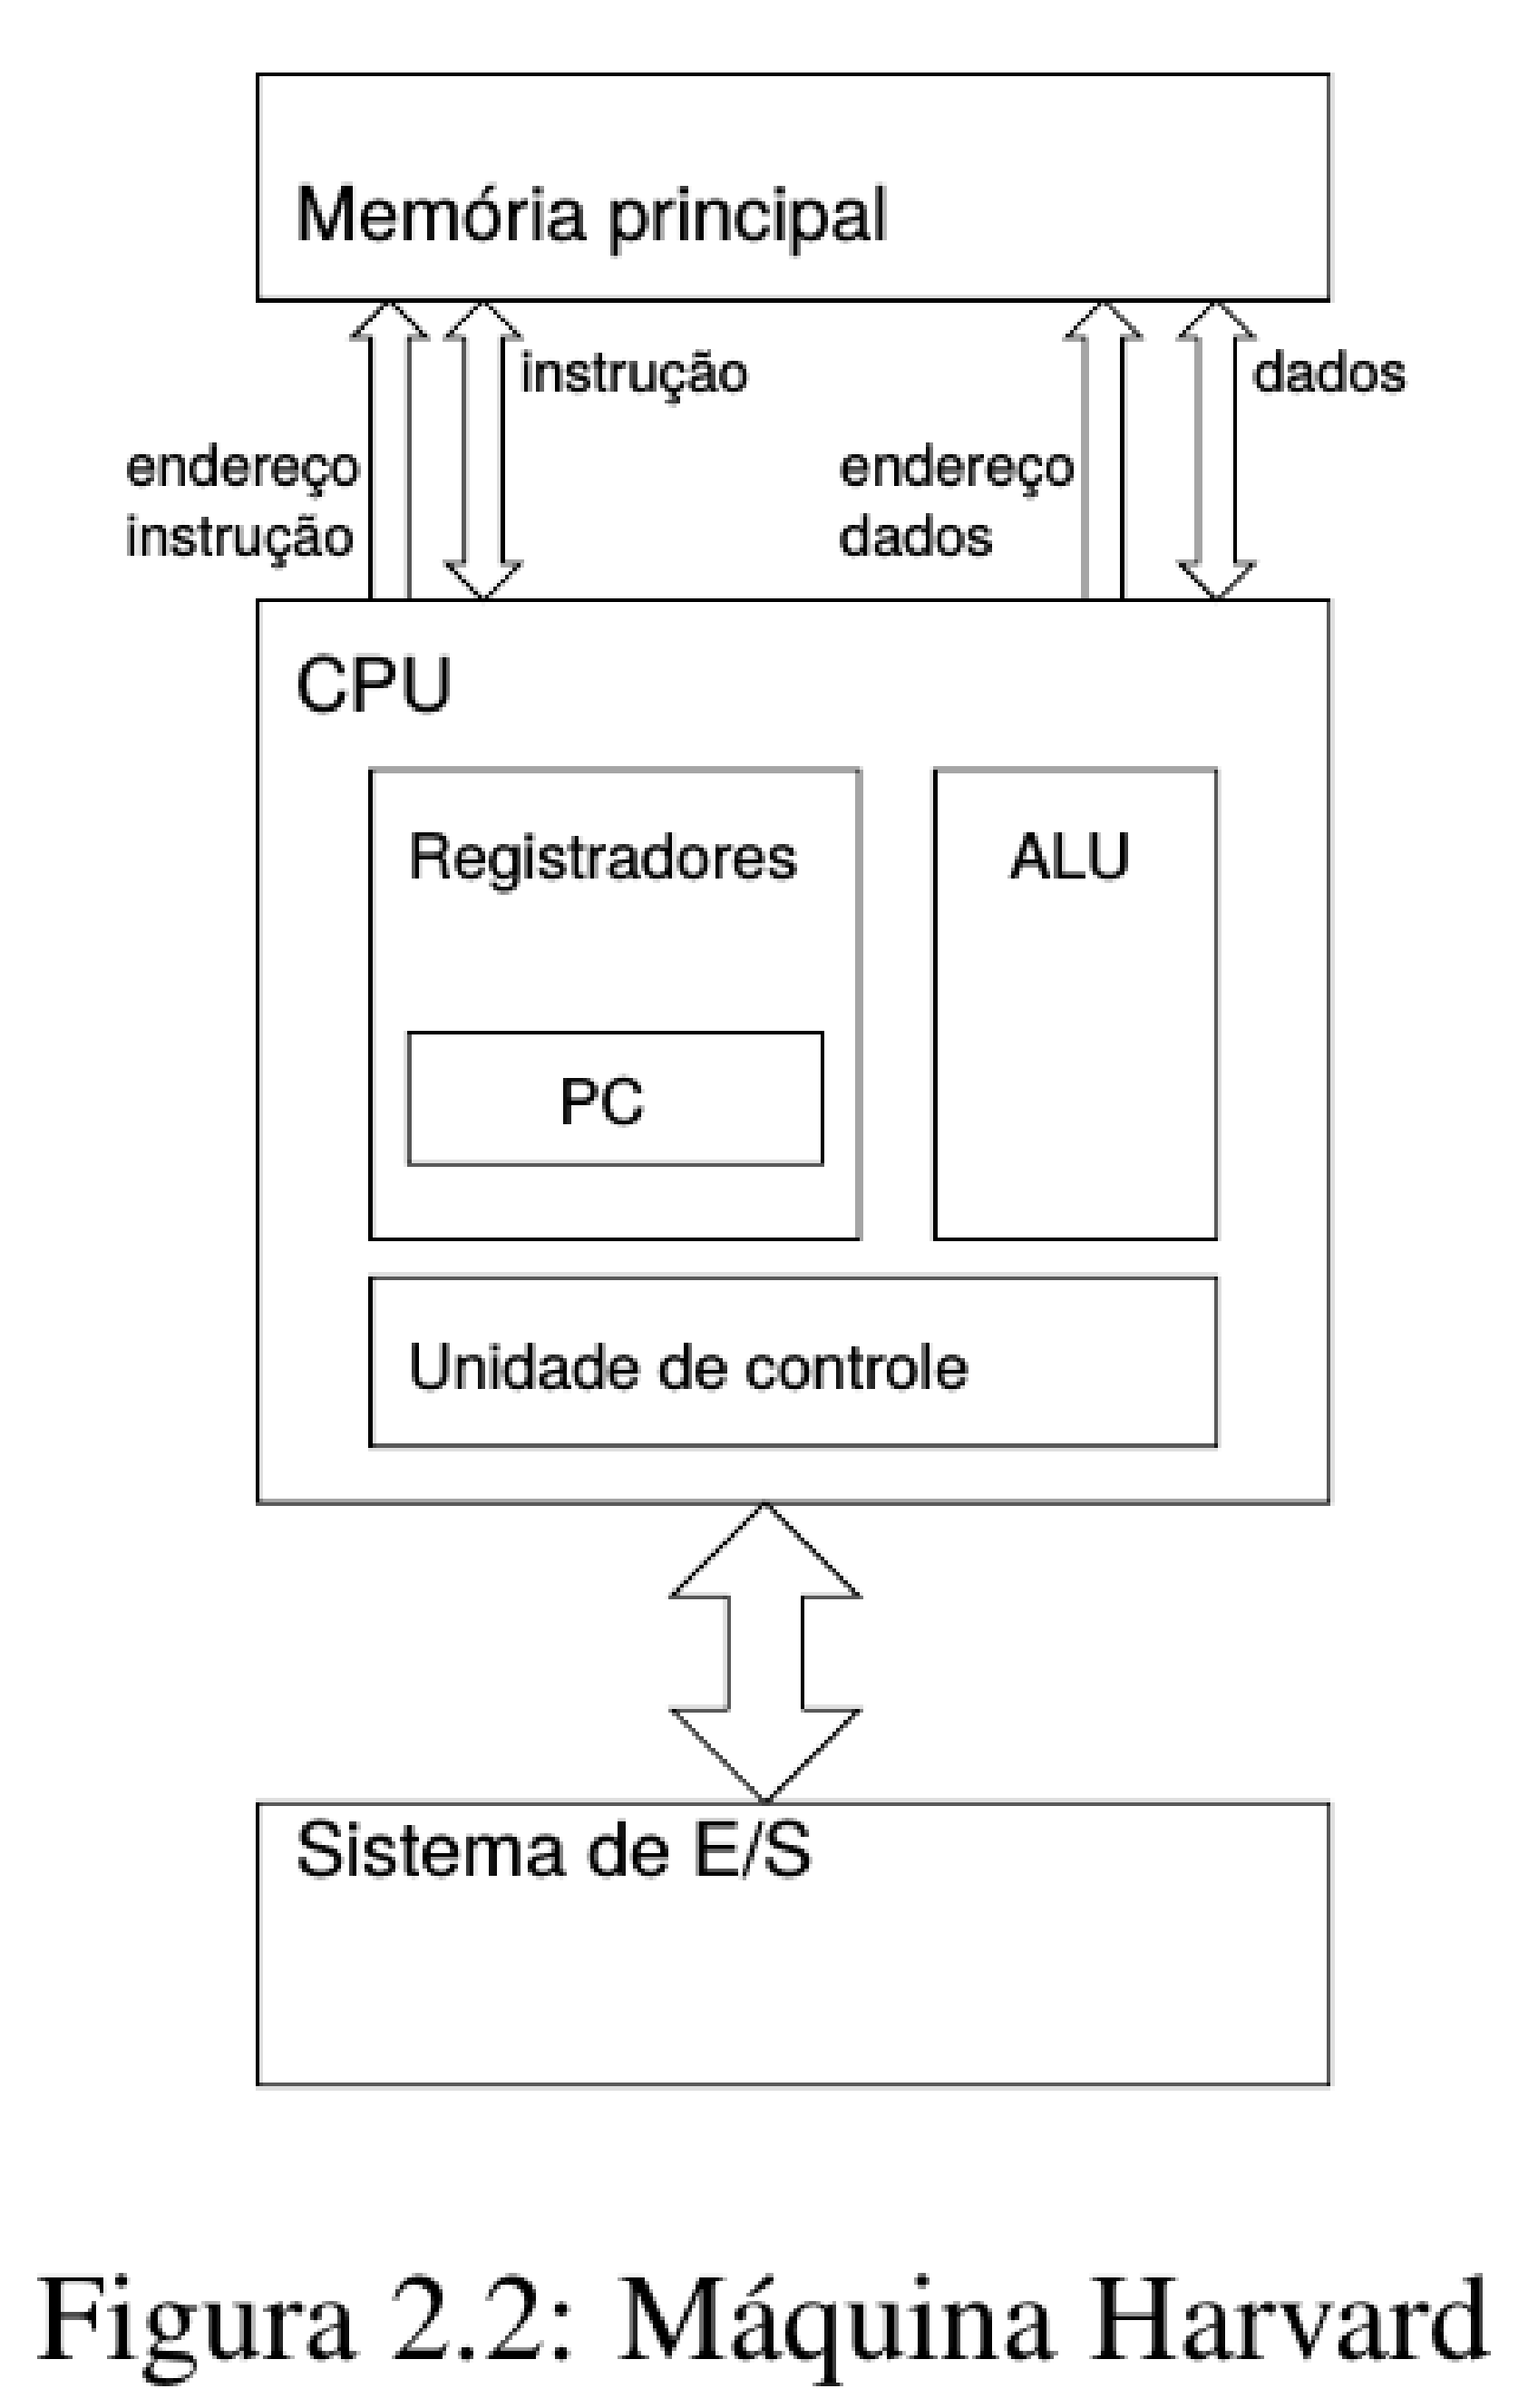
\includegraphics[width=0.8\textwidth]{images/vonnewman2.eps}
\end{center} 
\end{minipage}
\end{frame}

%%%%%%%%%%%%%%%%%%%%%%%%%%%%%%%%%%%%%%%%%%%%%%%%%%%%%%%%%%%%%%%%%%%%%%%%%%%%%%%%%
%https://www.youtube.com/watch?v=NmDdrI9ALxg
%https://en.wikibooks.org/wiki/Microprocessor_Design/Program_Counter
\begin{frame}{Exemplo de pipeline}
\begin{center}
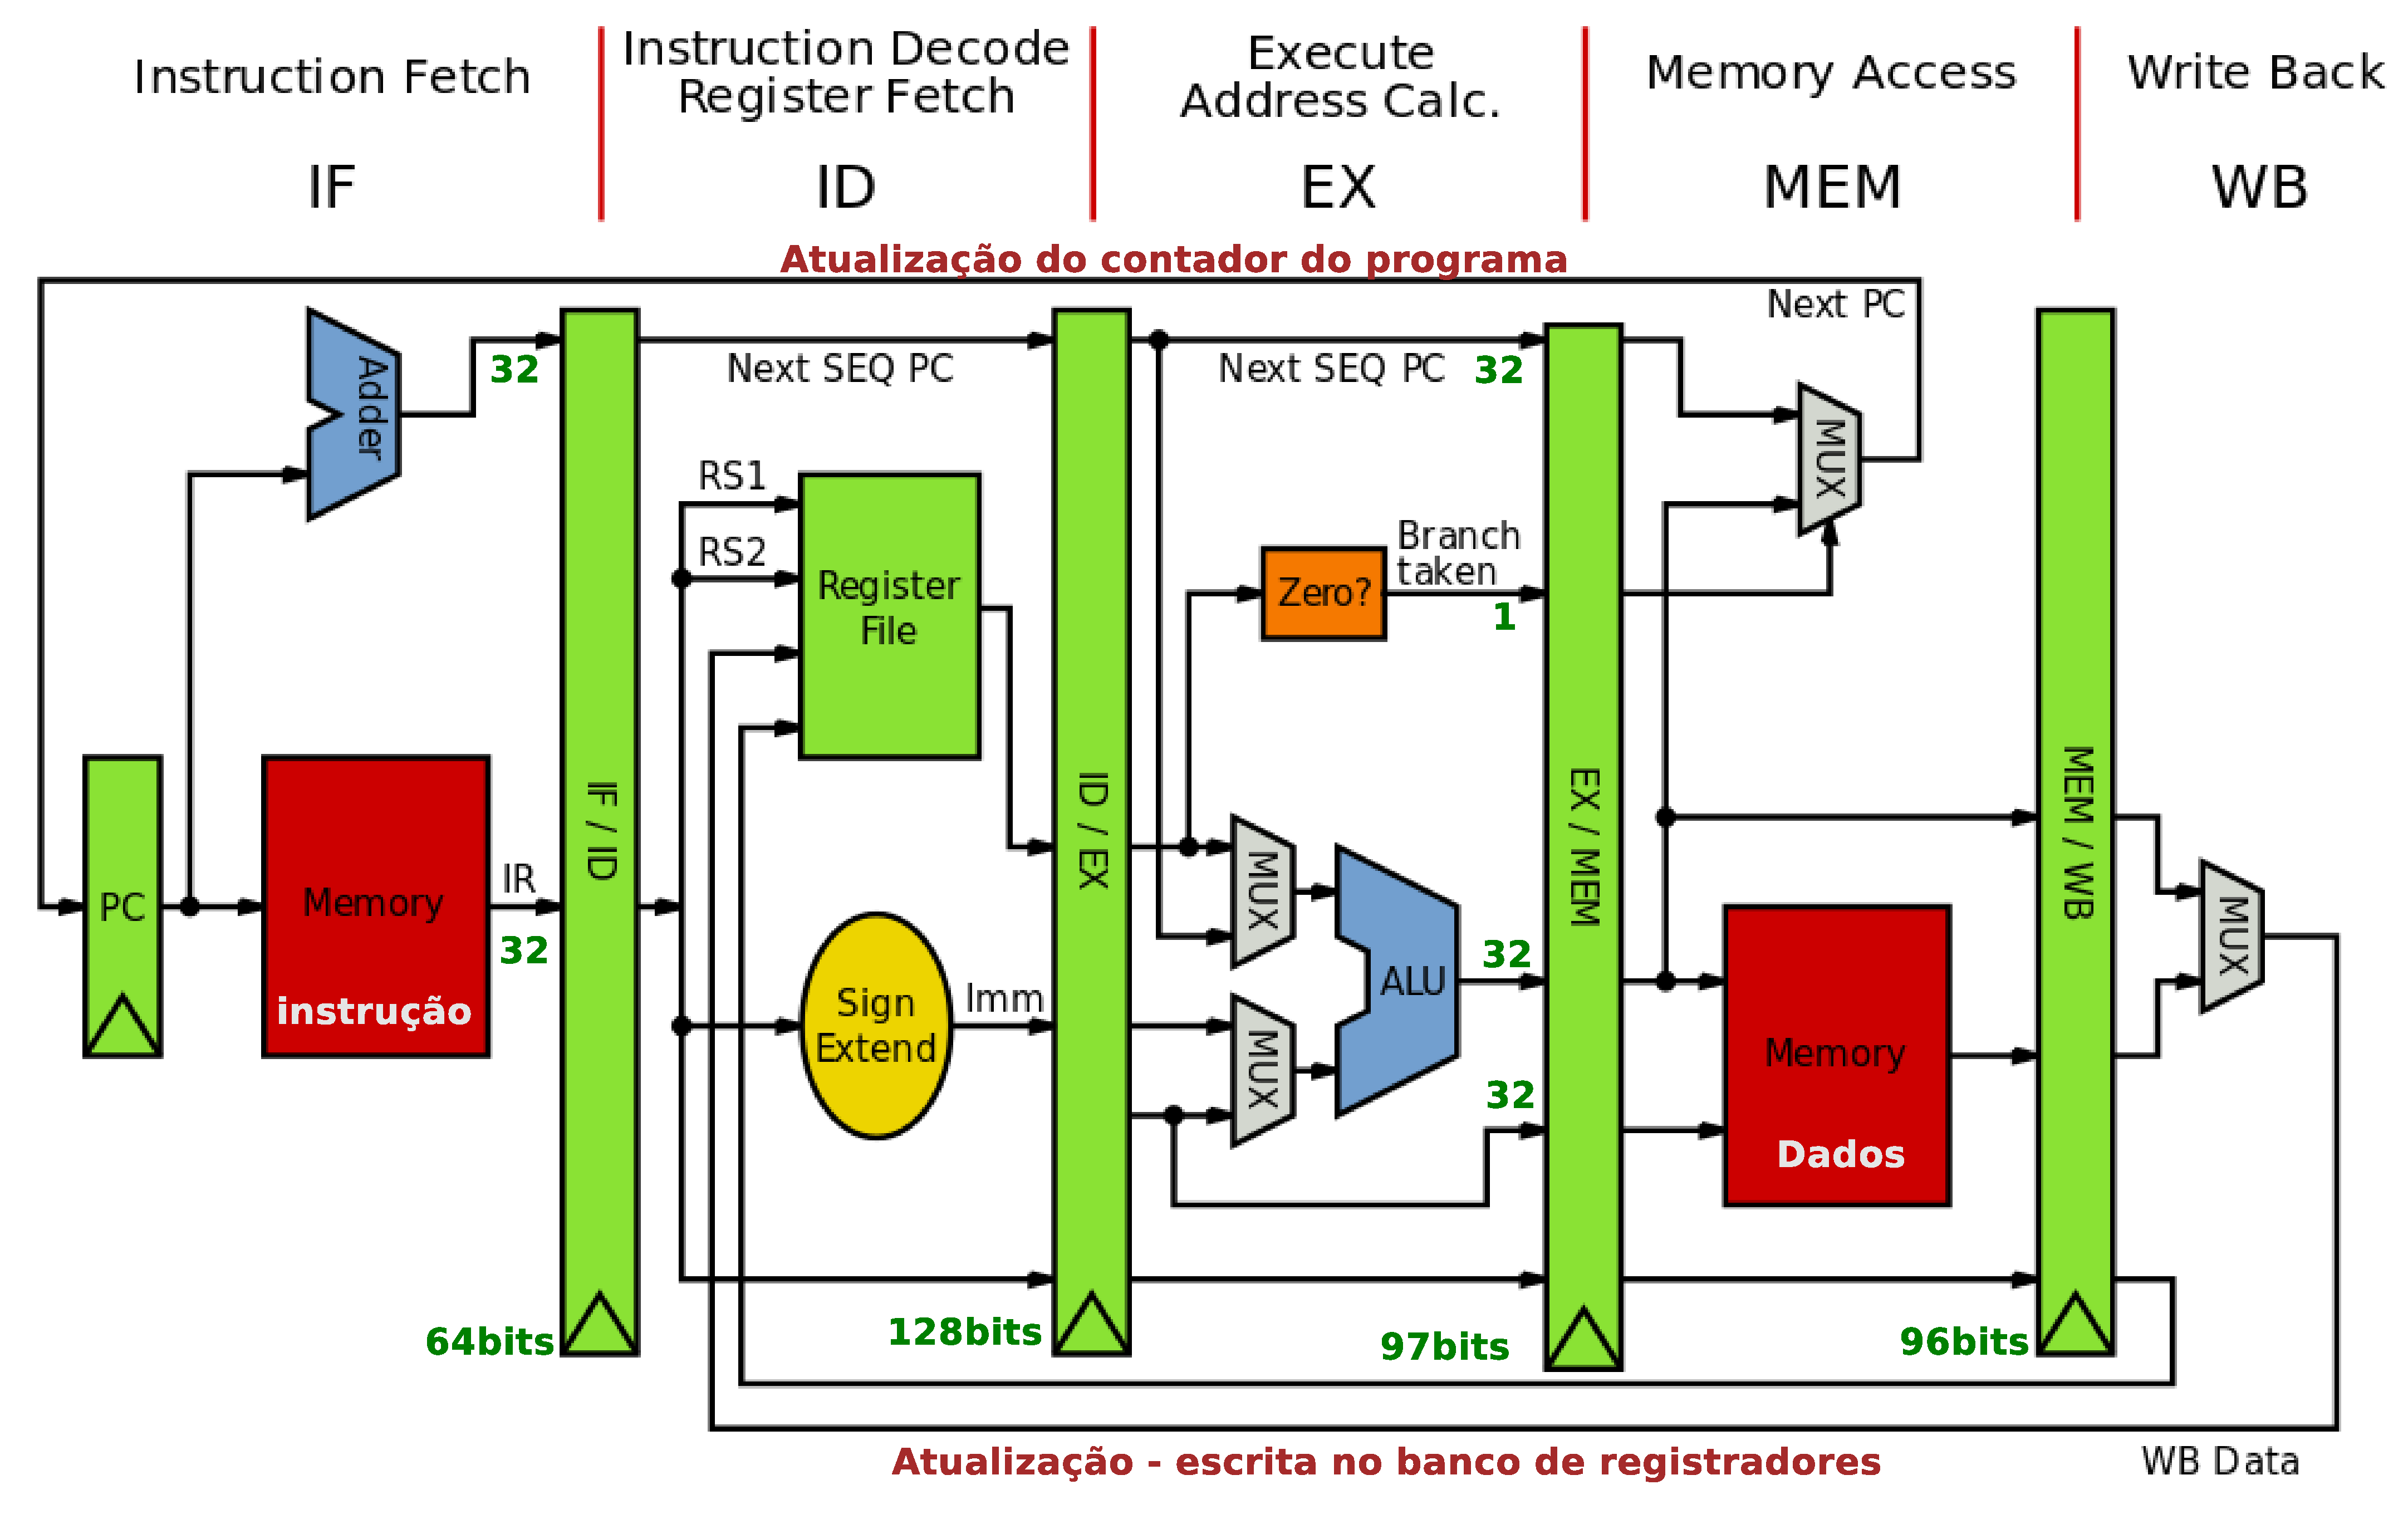
\includegraphics[width=1.0\textwidth]{images/MIPS_Architecture_(Pipelined).eps}
\end{center}
\end{frame}

%%%%%%%%%%%%%%%%%%%%%%%%%%%%%%%%%%%%%%%%%%%%%%%%%%%%%%%%%%%%%%%%%%%%%%%%%%%%%%%%%
%%%%%%%%%%%%%%%%%%%%%%%%%%%%%%%%%%%%%%%%%%%%%%%%%%%%%%%%%%%%%%%%%%%%%%%%%%%%%%%%%
\section{Conflitos}

%%%%%%%%%%%%%%%%%%%%%%%%%%%%%%%%%%%%%%%%%%%%%%%%%%%%%%%%%%%%%%%%%%%%%%%%%%%%%%%%%
% https://www.youtube.com/watch?v=-iQiruY4EBE
% https://www.youtube.com/watch?v=tcAbPJC_Qhs
% https://www.youtube.com/watch?v=hSOKxVX3vpw
\begin{frame}{Conflitos}
 \begin{block}{Conflitos}
\begin{description}
\item[Conflitos de recursos] Eu também preciso desse {\color{red}Hardware}. 
Também chamado de {\color{blue}conflito estrutural}.
\item[Conflitos de controle] {\color{red}Software}. Estes acontecem por desvios condicionais
(Ex: jne, jz Ex: if, while). A seguinte instrução no FETCH é desconhecida ate
EX da instrução anterior.
\item[Conflitos de dados] {\color{red}Software}. Duas instruções estão lendo
e escrevendo sobre o mesmo dado.
\end{description}
\end{block}
A forma mais fácil de resolver conflitos é agregando pausas. Mas é pouco recomendável.
\end{frame}

%%%%%%%%%%%%%%%%%%%%%%%%%%%%%%%%%%%%%%%%%%%%%%%%%%%%%%%%%%%%%%%%%%%%%%%%%%%%%%%%%
\begin{frame}{Conflitos de recursos}
\begin{description}
 \item[Acesso à memória:] Ler e escrever na memória ao mesmo tempo (Von Newmann)
 \item[Unidades de execução:]  Usar a ALU simultaneamente (Ex: incremento de PC e operação aritmética).
\end{description}
\begin{minipage}[c]{0.5\textwidth}
\begin{center}
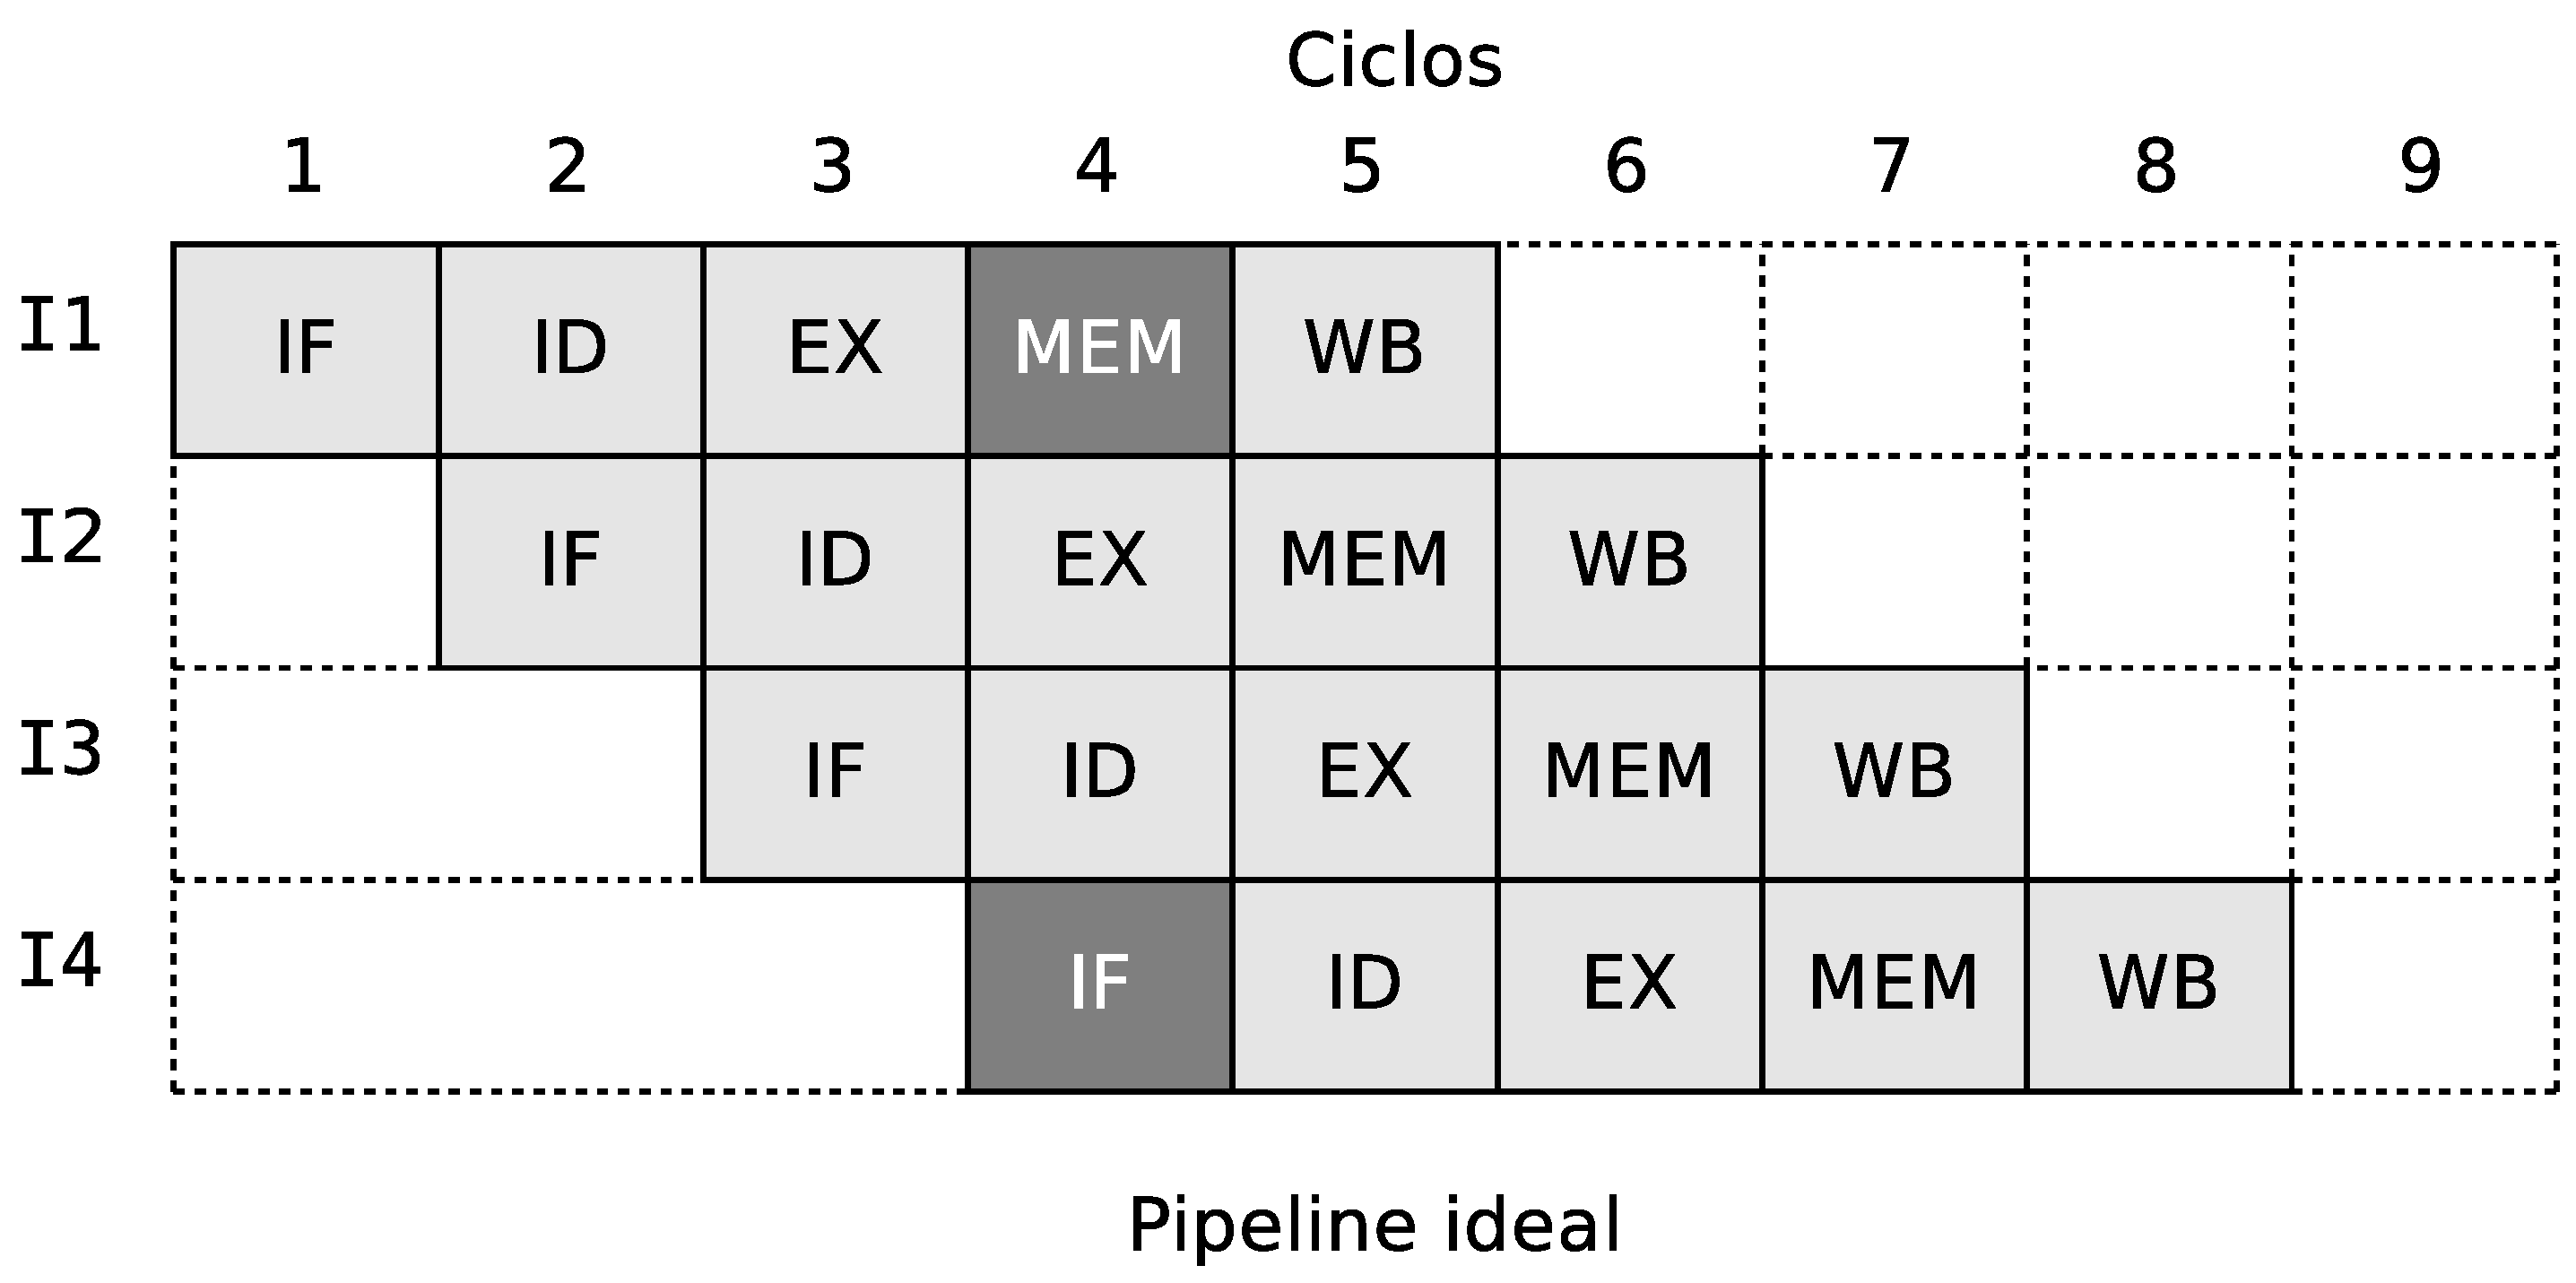
\includegraphics[width=0.9\textwidth]{images/diagrama1.eps}
\end{center} 
\end{minipage}%
\begin{minipage}[c]{0.5\textwidth}
\begin{center}
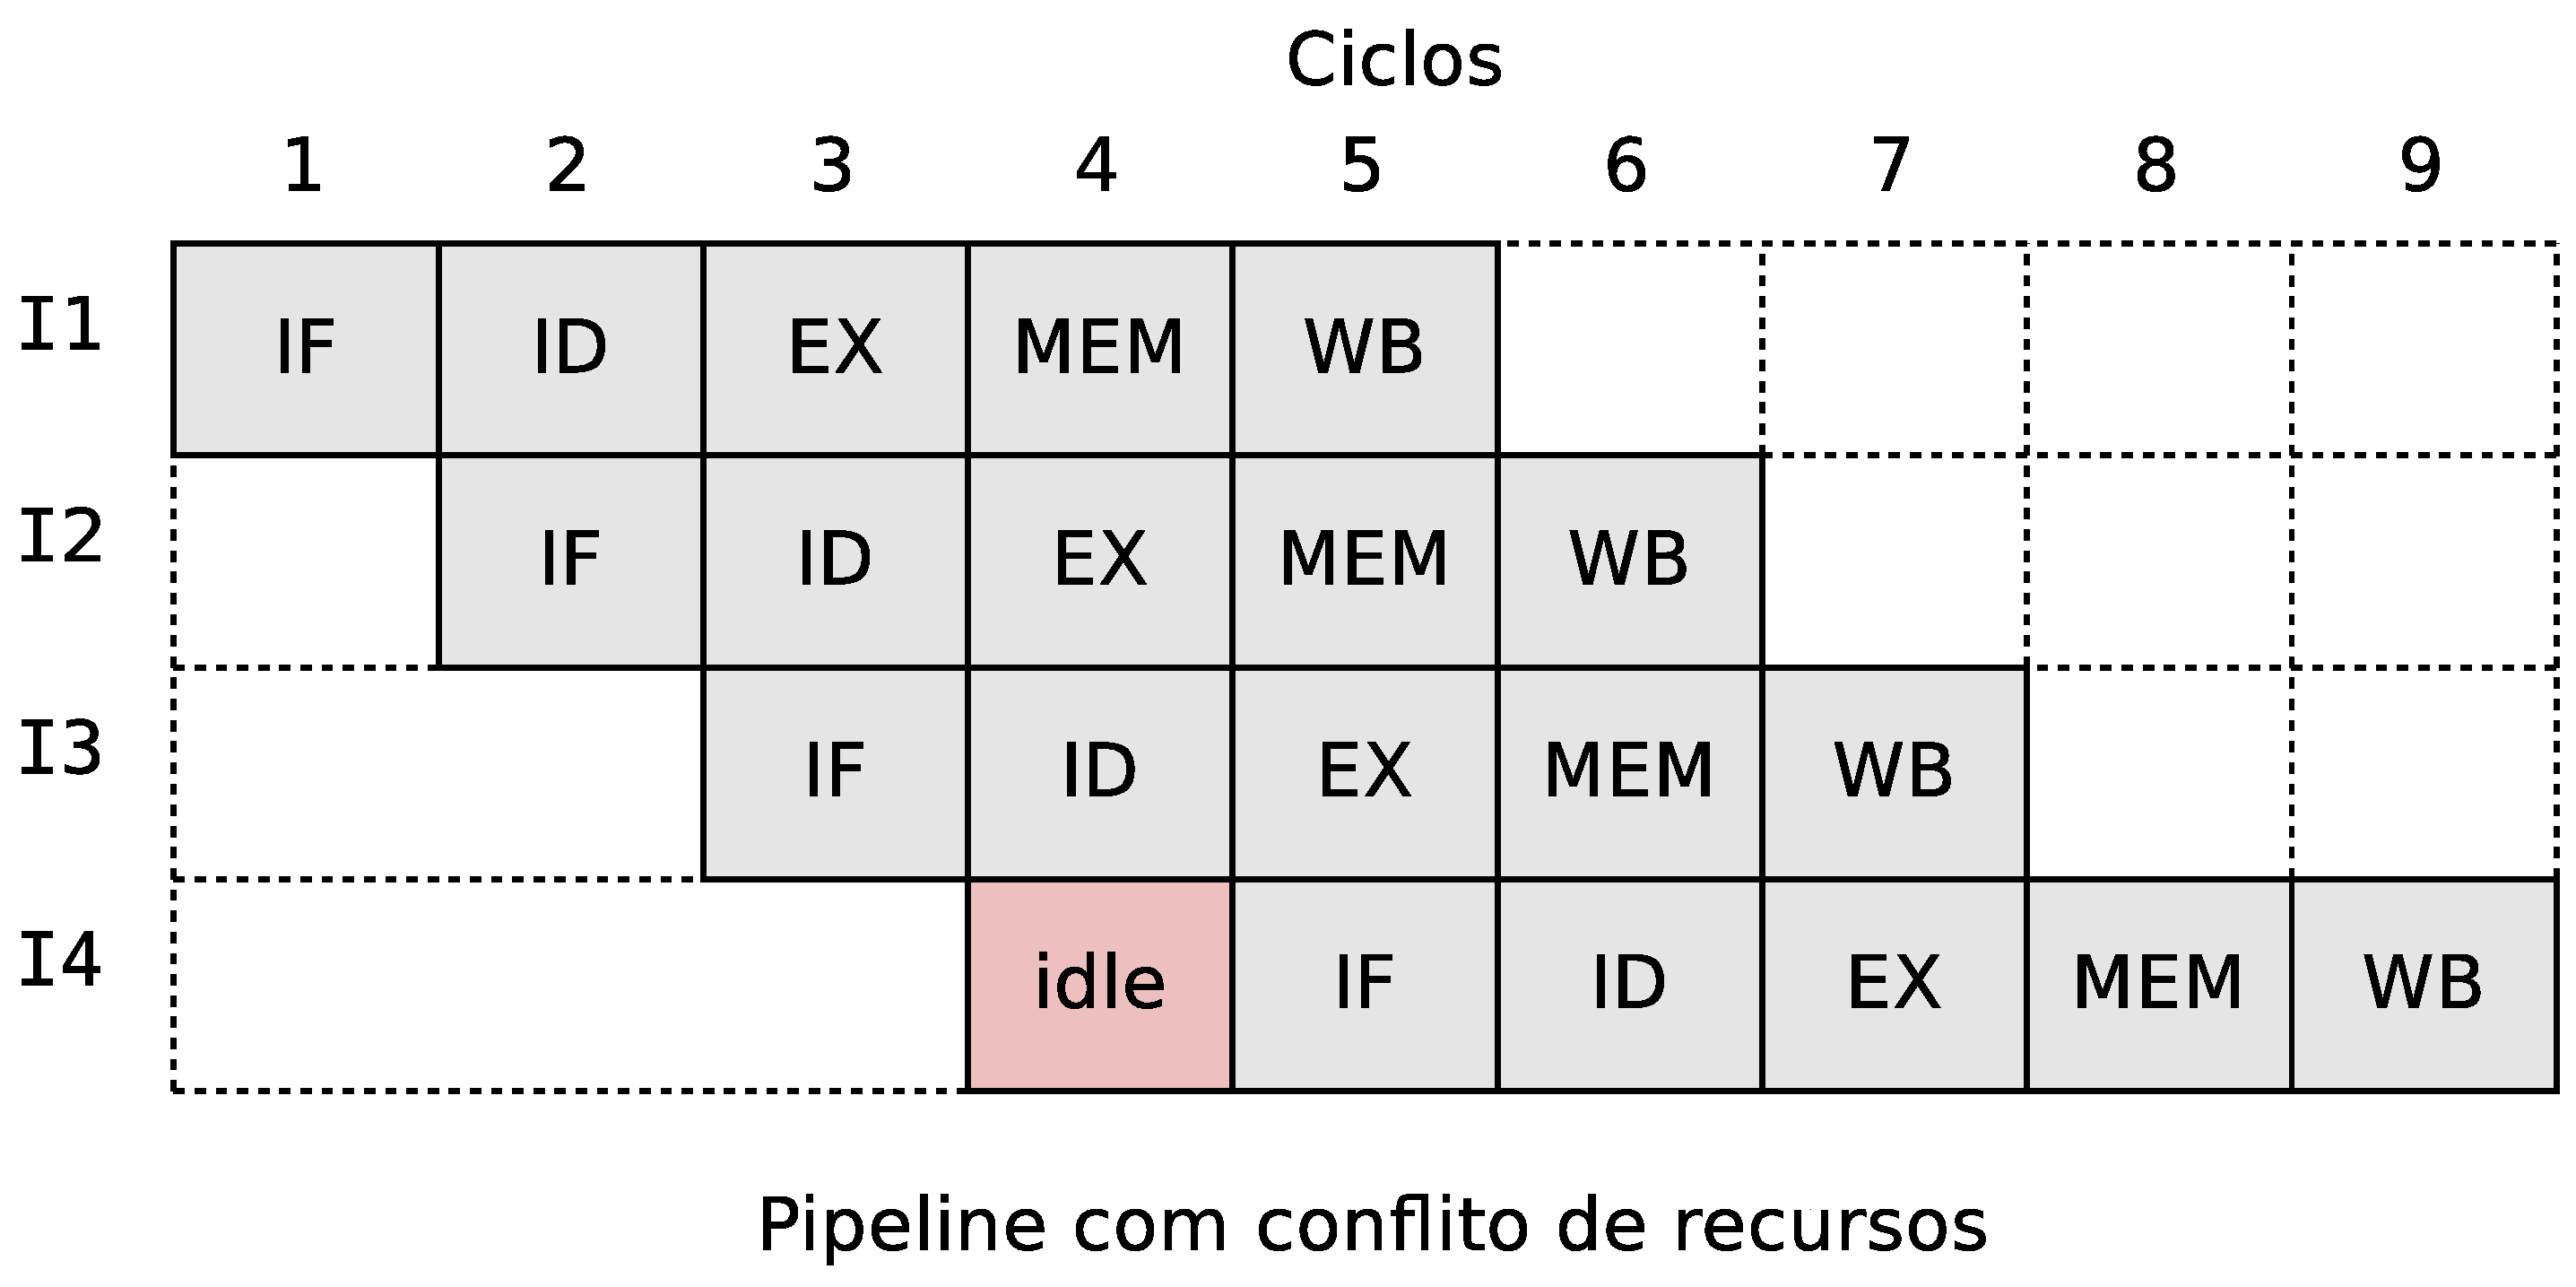
\includegraphics[width=0.9\textwidth]{images/diagrama2.eps}
\end{center} 
\end{minipage}

\begin{minipage}[c]{0.3\textwidth}
\begin{center}
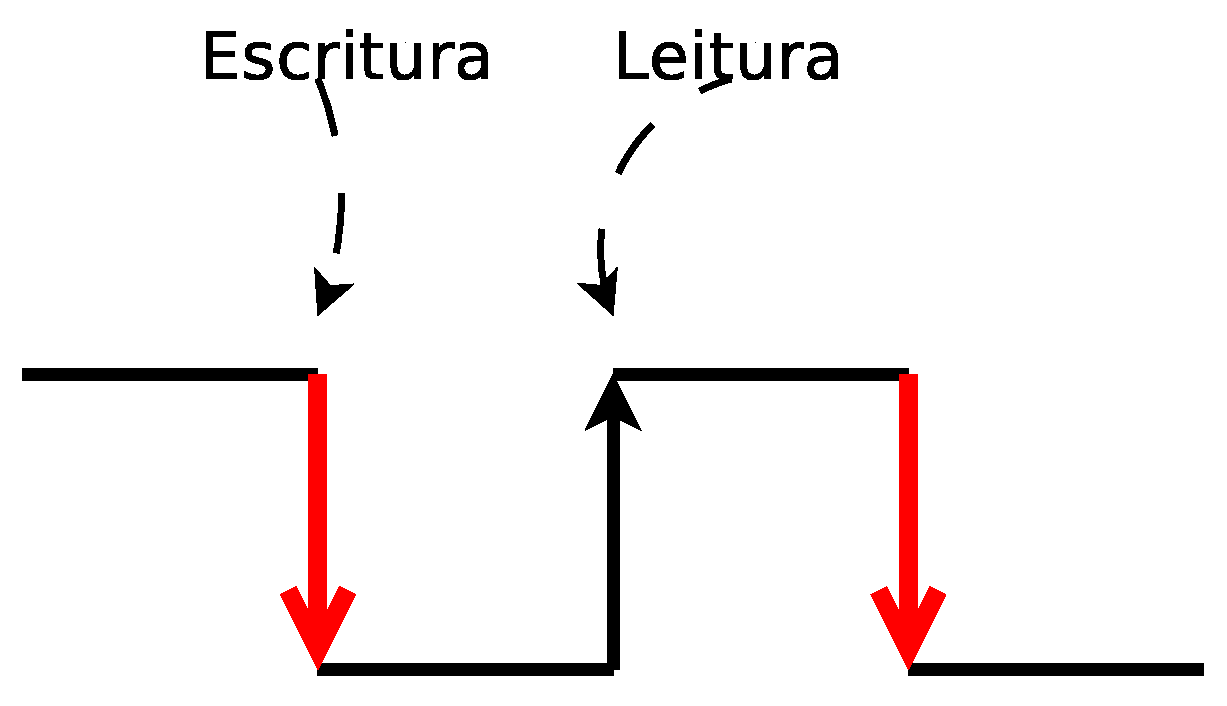
\includegraphics[width=0.9\textwidth]{images/ciclo.eps}
\end{center} 
\end{minipage}%
\begin{minipage}[c]{0.7\textwidth}
Solução: 2 Caches, instruções e dados .Distribuir melhor os tempos. Incrementar a quantidade de recursos; memoria, ALU. 
\end{minipage}
\end{frame}


%%%%%%%%%%%%%%%%%%%%%%%%%%%%%%%%%%%%%%%%%%%%%%%%%%%%%%%%%%%%%%%%%%%%%%%%%%%%%%%%%
% http://pt.slideshare.net/carlossergiosjp/arquitetura-e-organizao-de-computadores-1-pipeline
% http://homepage.cs.uiowa.edu/~ghosh/4-20-10.pdf
\begin{frame}{Conflitos de controle}
\begin{center}
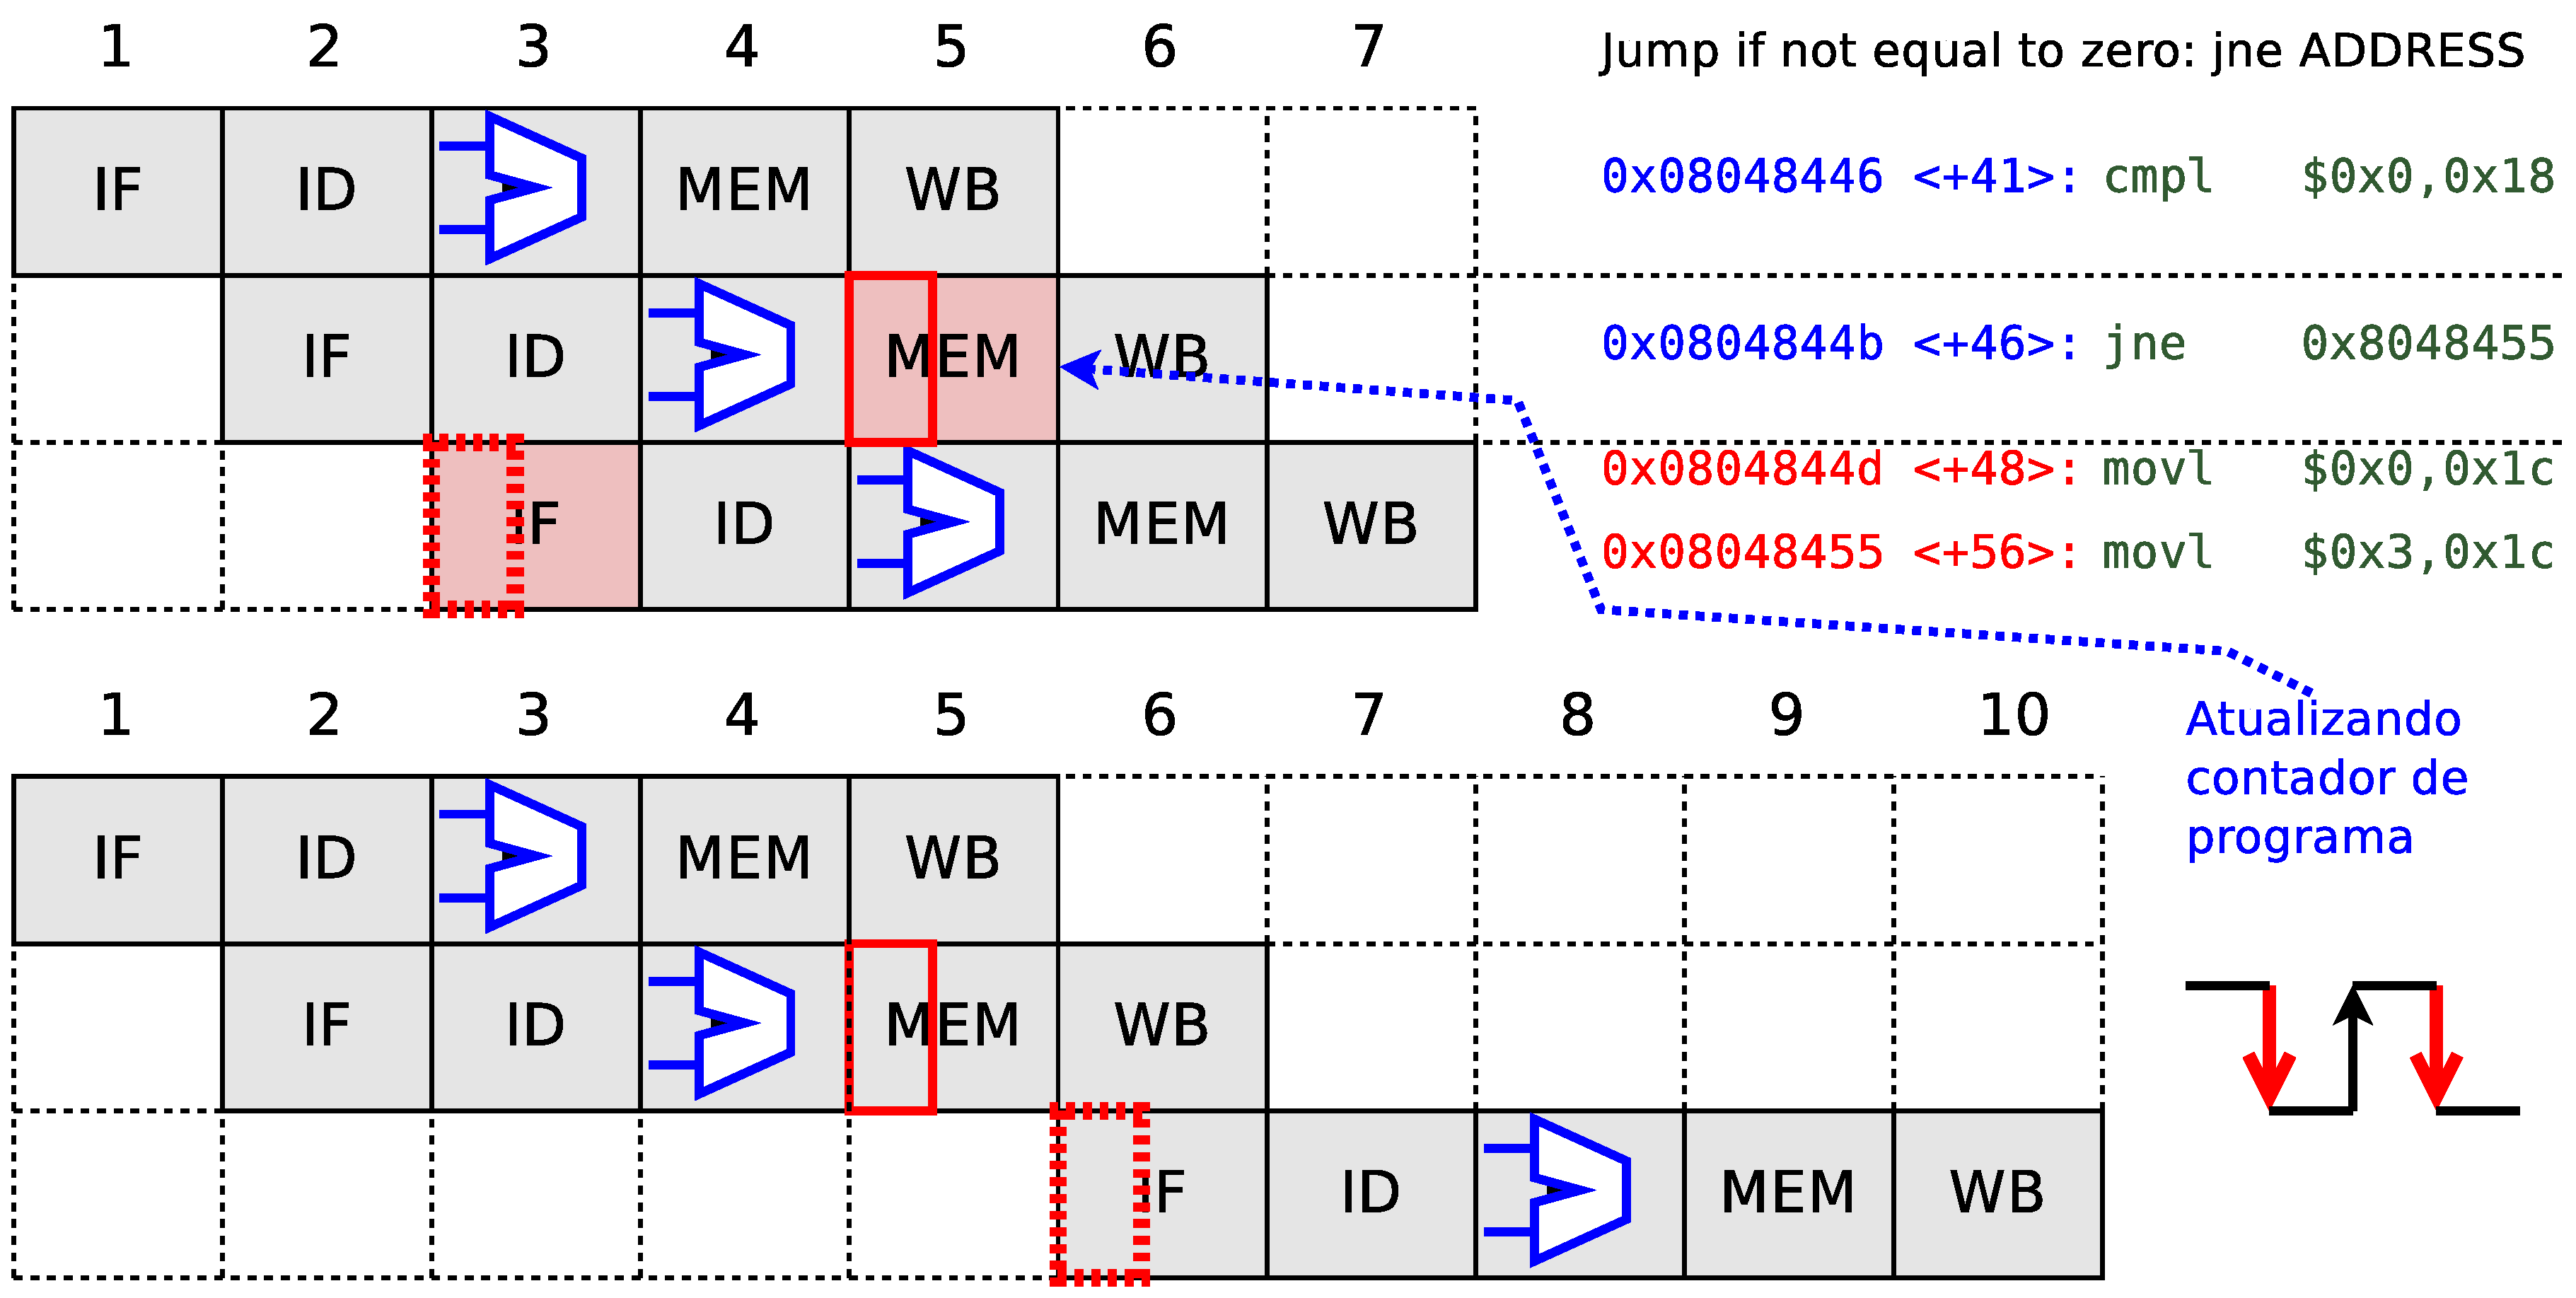
\includegraphics[width=0.9\textwidth]{images/conflitocontrole.eps}
\end{center} 
\end{frame}
\begin{frame}{Conflitos de controle}
\begin{description}
 \item[Técnica de previsão estática:] Simples: Sempre assumir FALSE no desvio condicional. 
 Sofisticada: Assumir que se o anterior desviou para lá, agora também.
 \item[Técnica de previsão dinâmica:] Estatística do prox. endereço (2 possíveis), 
 FETCH recebe a instrução mais provável. Precisa de etapa de controle para descartar
 previsões erradas.
\item[Retardar instruções:]  Interlock: a entrada (FETCH) é bloqueada ate resolver o desvio. 
Ou mandamos a fazer algo útil (compilador).
\end{description}
\end{frame}

%%%%%%%%%%%%%%%%%%%%%%%%%%%%%%%%%%%%%%%%%%%%%%%%%%%%%%%%%%%%%%%%%%%%%%%%%%%%%%%%%
% https://www.youtube.com/watch?v=hSOKxVX3vpw
% ftp://ftp.dca.fee.unicamp.br/pub/docs/ea960/ea960.pdf
\begin{frame}{Conflitos de dados}
\begin{block}{Conflitos de dados}
Quando operandos de uma instrução dependem do resultado de uma instrução anterior
\end{block}
\begin{center}
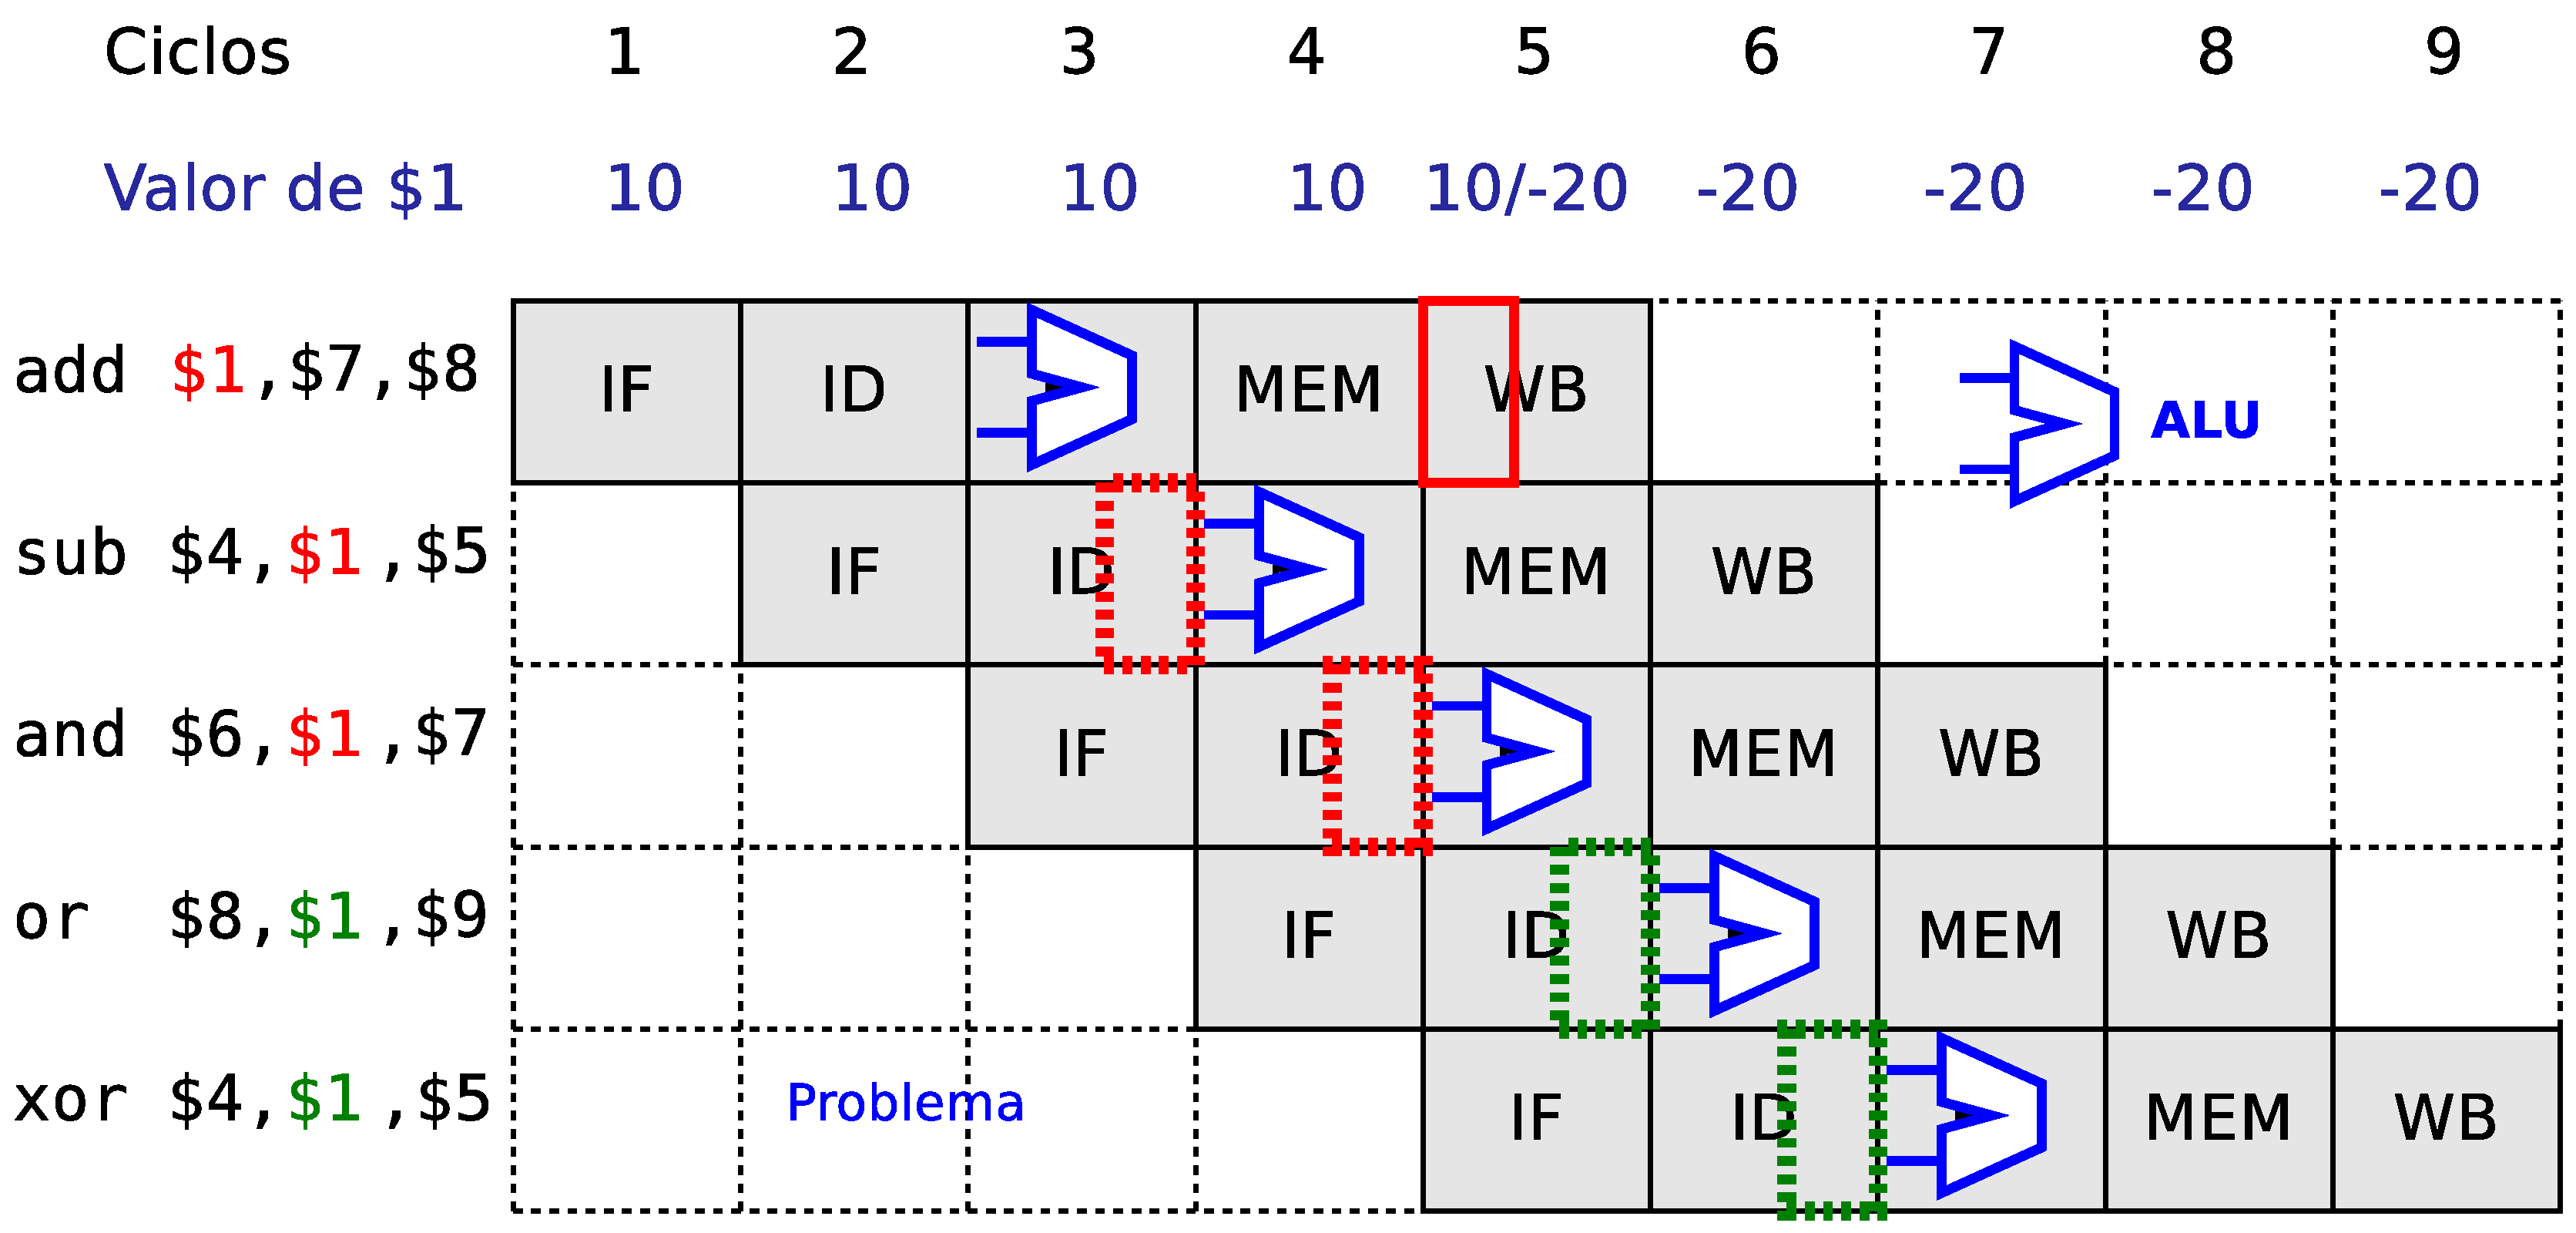
\includegraphics[width=0.9\textwidth]{images/conflitodados1.eps}
\end{center} 
\end{frame}
\begin{frame}{Conflitos de dados}
\begin{block}{Conflitos de dados}
Quando operandos de uma instrução dependem do resultado de uma instrução anterior
\end{block}
\begin{center}
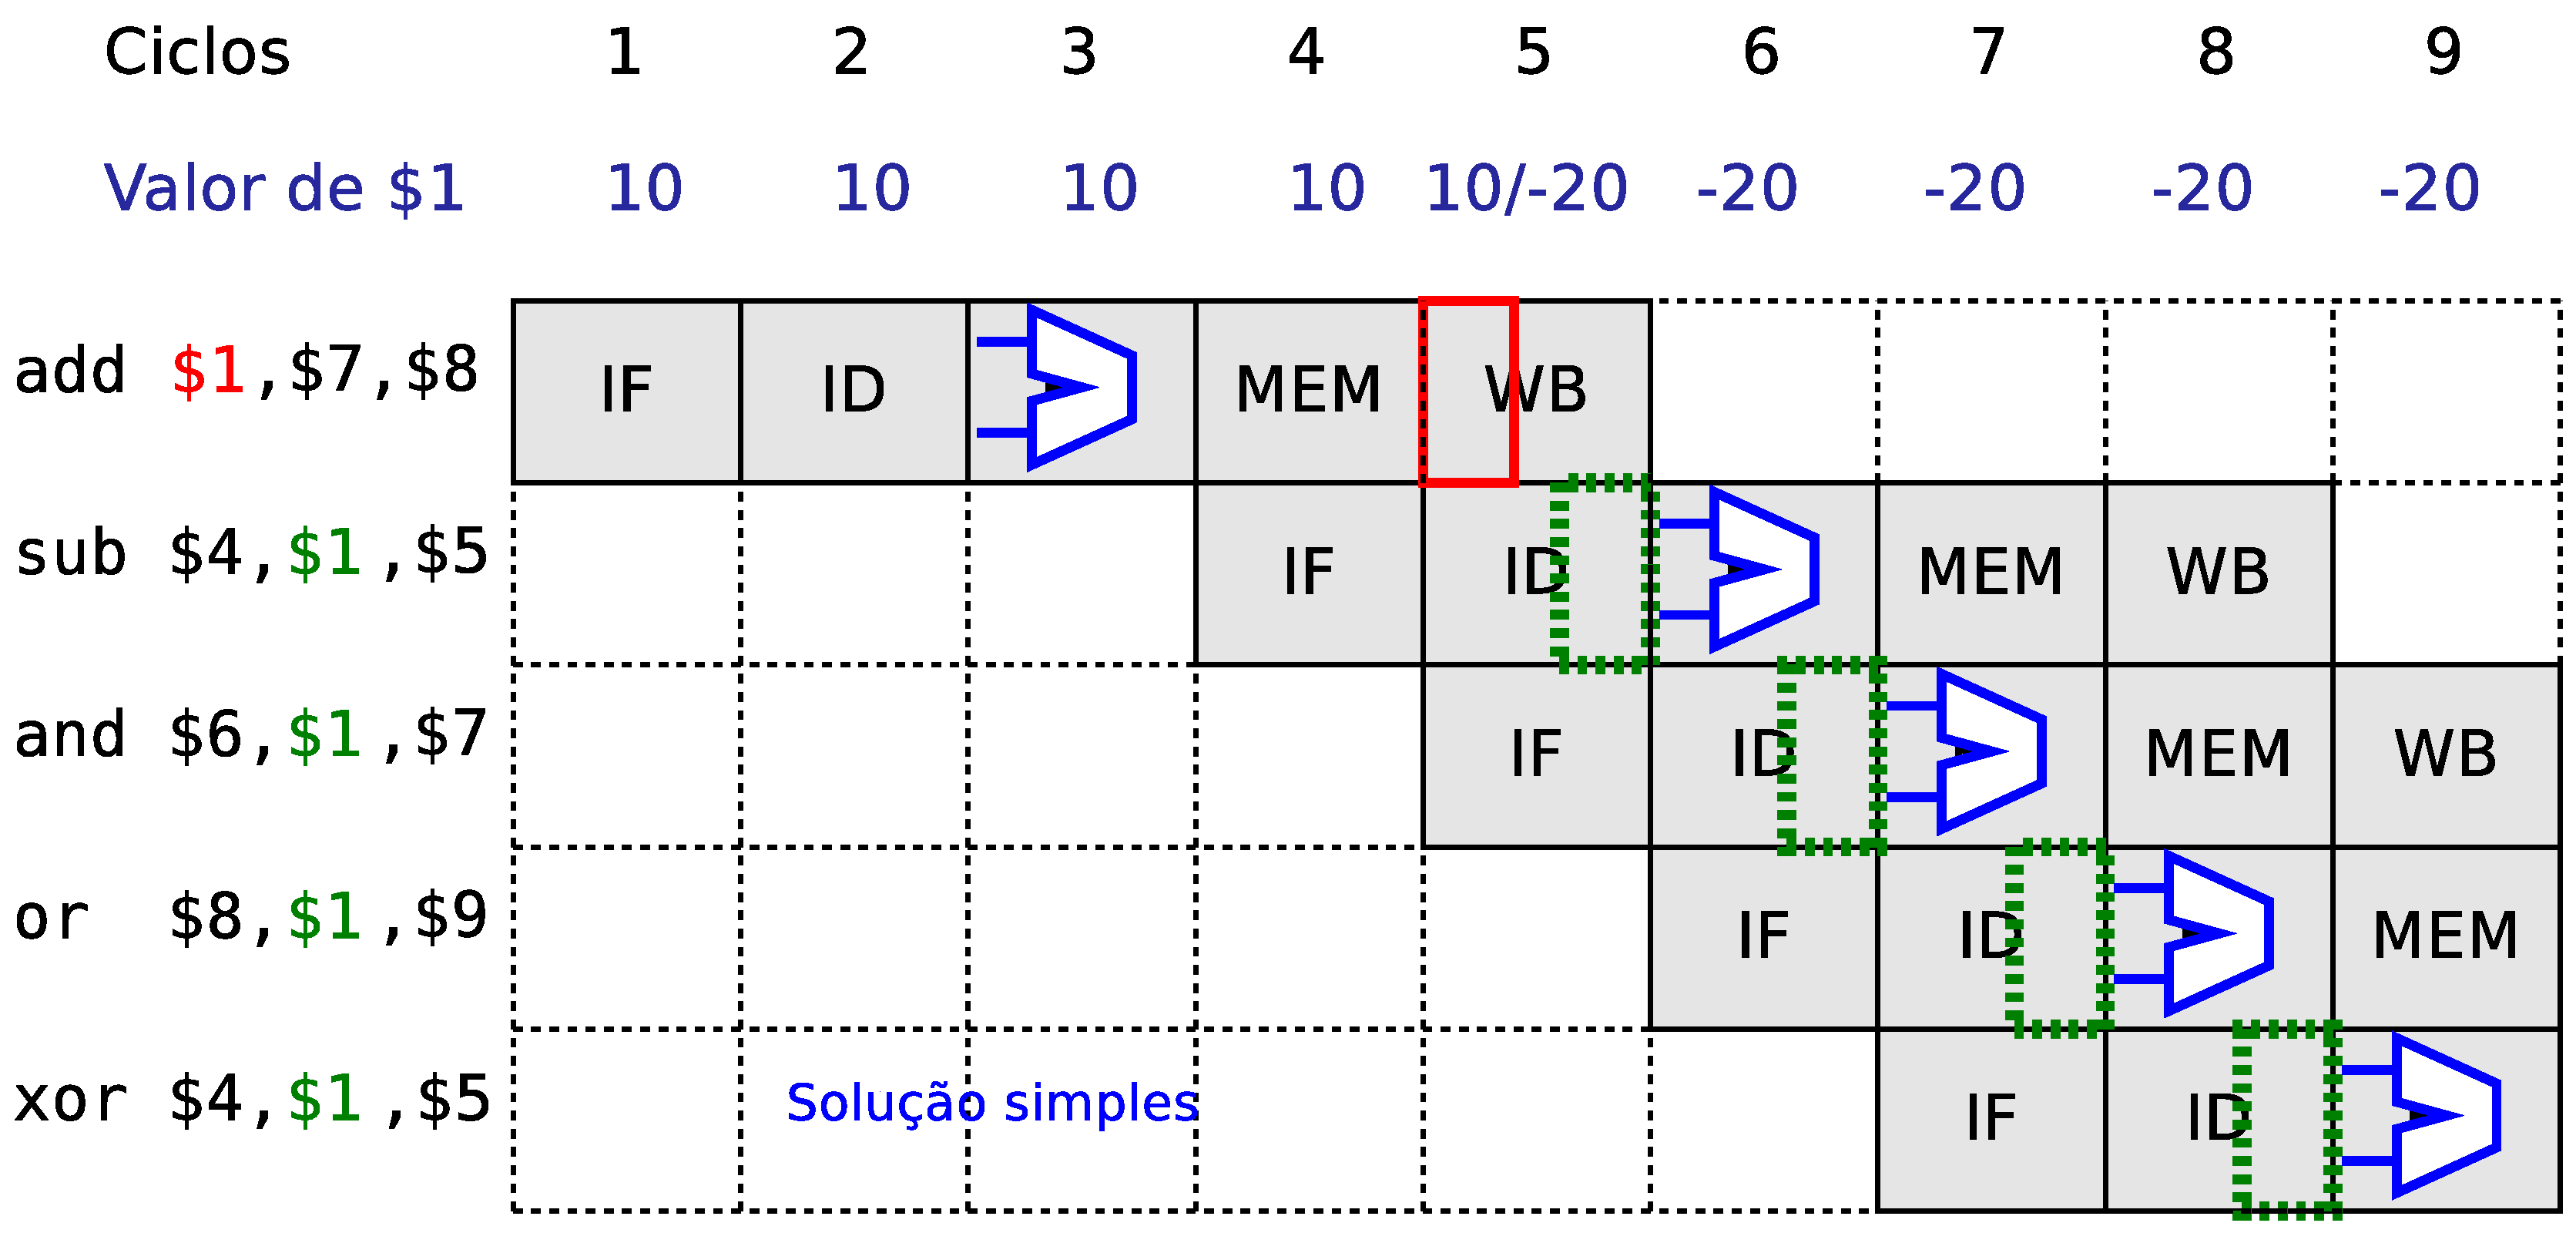
\includegraphics[width=0.9\textwidth]{images/conflitodados2.eps}
\end{center} 
\end{frame}
\begin{frame}{Conflitos de dados}
\begin{block}{Conflitos de dados}
Quando operandos de uma instrução dependem do resultado de uma instrução anterior
\end{block}
\begin{center}
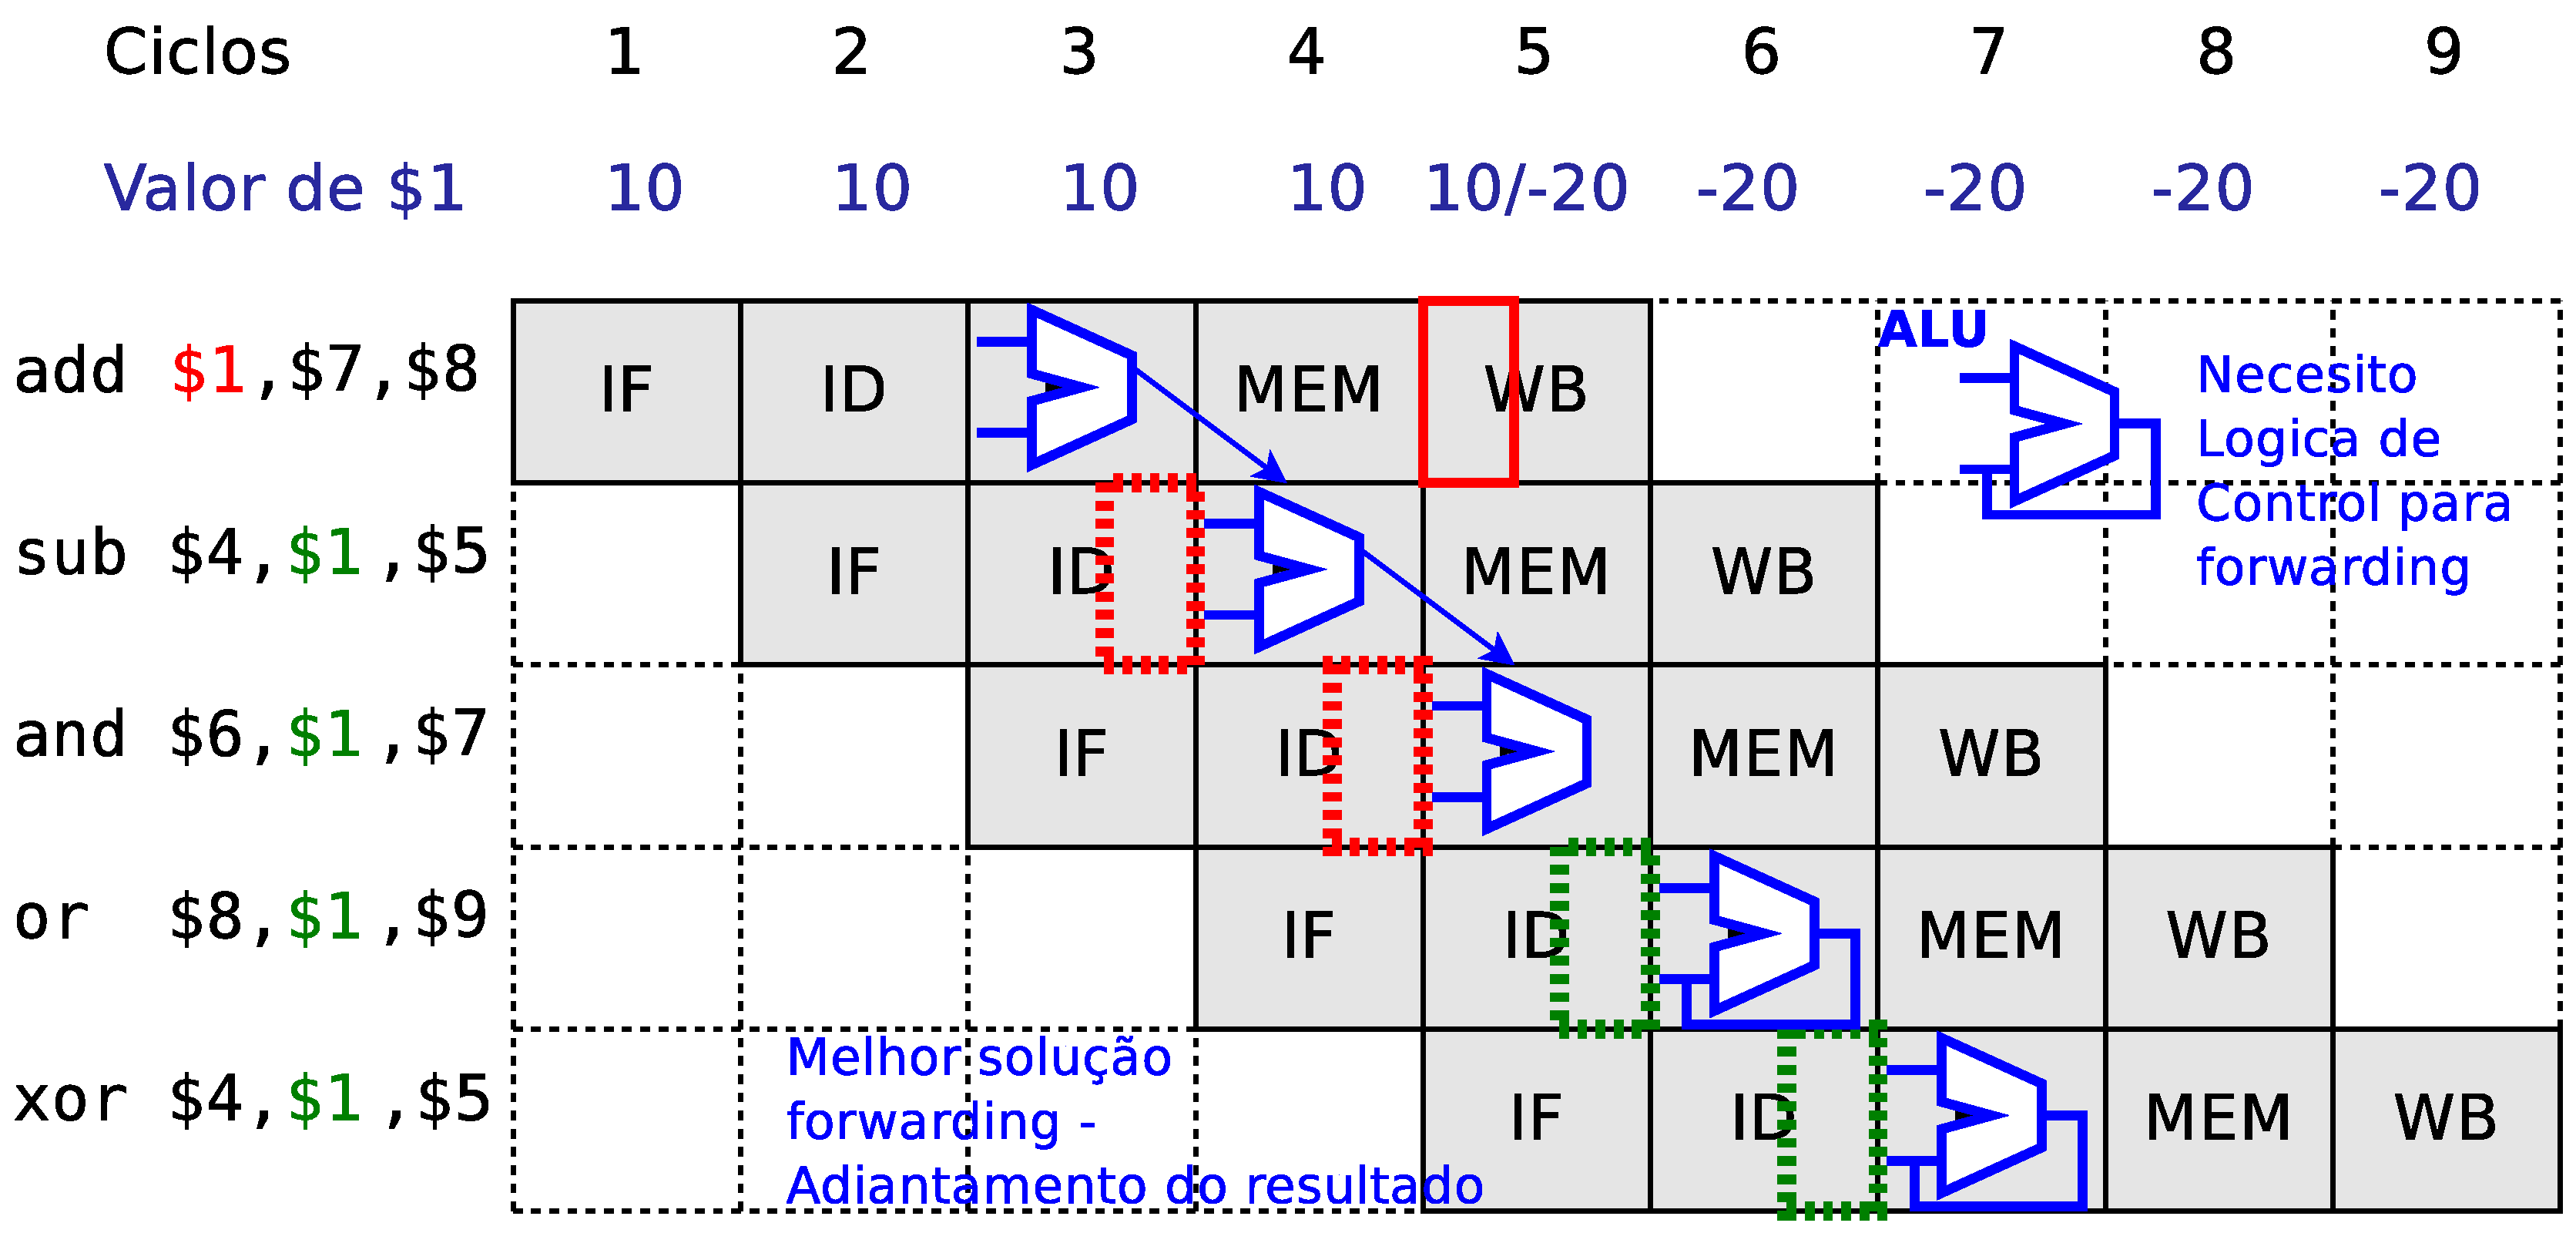
\includegraphics[width=0.9\textwidth]{images/conflitodados3.eps}
\end{center} 
\end{frame}

%%%%%%%%%%%%%%%%%%%%%%%%%%%%%%%%%%%%%%%%%%%%%%%%%%%%%%%%%%%%%%%%%%%%%%%%%%%%%%%%
\begin{frame}[allowframebreaks]
        \frametitle{References}
        \bibliographystyle{plain}
\bibliography{pipeline}
\end{frame}



\end{document}
